\chapter{Analisis}
\label{chap:analisis}

\section{Tingkat Kepatuhan \textit{SharIF Judge}}
\label{sec:kepatuhan_sharif_judge_terhadap_wcag_2.1}
Kesuksesan aplikasi SharIF Judge dalam mematuhi kriteria sukses \textit{WCAG} 2.1 ditulis dalam tabel-tabel berikut.

\begin{table}[H]
	\centering
	\caption{Tabel kepatuhan \textit{SharIF Judge} terhadap prinsip \textit{Perceivable}}
	\label{tab:kepatuhan_sharif_judge_perceivable}
	\begin{tabular}{|c|c|c|}
		\hline
		Kriteria Sukses & Tingkat Kepatuhan & Hasil \\
		\hline
		1.1.1 & A & Tidak Sukses \\
		1.2.1 & A & Sukses \\
		1.2.2 & A & Sukses \\
		1.2.3 & A & Sukses \\
		1.2.4 & AA & Sukses \\
		1.2.5 & AA & Sukses \\
		1.2.6 & AAA & Sukses \\
		1.2.7 & AAA & Sukses \\
		1.2.8 & AAA & Sukses \\
		1.2.9 & AAA & Sukses \\
		1.3.1 & A & Tidak Sukses\\
		1.3.2 & A & Sukses \\
		1.3.3 & A & Sukses \\
		1.3.4 & A & Sukses \\
		1.3.5 & AA & Tidak Sukses \\
		1.3.6 & AAA & Tidak Sukses \\
		1.4.1 & A & Sukses \\
		1.4.2 & A & Sukses \\
		1.4.3 & AA & Tidak Sukses \\
		1.4.4 & AA & Tidak Sukses \\
		1.4.5 & AA & Sukses \\
		1.4.6 & AAA & Tidak Sukses \\
		1.4.7 & AAA & Sukses \\
		1.4.8 & AAA & Tidak Sukses \\
		1.4.9 & AAA & Sukses \\
		1.4.10 & AA & Tidak Sukses \\
		1.4.11 & AA & Diabaikan \\
		1.4.12 & AA & \\
		1.4.13 & AA & Sukses \\
		\hline
	\end{tabular}
\end{table}

\begin{table}[H]
	\centering
	\caption{Tabel kepatuhan \textit{SharIF Judge} terhadap prinsip \textit{Operable}}
	\label{tab:kepatuhan_sharif_judge_operable}
	\begin{tabular}{|c|c|c|}
		\hline
		Kriteria Sukses & Tingkat Kepatuhan & Hasil \\
		\hline
		2.1.1 & A & Tidak Sukses \\
		2.1.2 & A & Tidak Sukses \\
		2.1.3 & AAA & Tidak Sukses \\
		2.1.4 & A & Sukses \\
		2.2.1 & A & Sukses \\
		2.2.2 & A & Sukses \\
		2.2.3 & AAA & Sukses \\
		2.2.4 & AAA & Sukses \\
		2.2.5 & AAA & Tidak Sukses \\
		2.2.6 & AAA & Tidak Sukses \\
		2.3.1 & A & Sukses\\
		2.3.2 & AAA & Sukses\\
		2.3.3 & AAA & Sukses\\
		2.4.1 & A & Tidak Sukses\\
		2.4.2 & A & Sukses \\
		2.4.3 & A & Sukses \\
		2.4.4 & A & Tidak Sukses \\
		2.4.5 & AA & Tidak Sukses \\
		2.4.6 & AA & Tidak Sukses \\
		2.4.7 & AA & Tidak Sukses\\
		2.4.8 & AAA & Sukses\\
		2.4.9 & AAA & Tidak Sukses\\
		2.4.10 & AAA & Tidak Sukses\\
		2.5.1 & A & Sukses\\
		2.5.2 & A & Sukses\\
		2.5.3 & A & Tidak Sukses\\
		2.5.4 & A & Sukses\\
		2.5.5 & AAA & Tidak Sukses\\
		2.5.6 & AAA & Sukses\\
		\hline
	\end{tabular}
\end{table}

\begin{table}[H]
	\centering
	\caption{Tabel kepatuhan \textit{SharIF Judge} terhadap prinsip \textit{Understandable}}
	\label{tab:kepatuhan_sharif_judge_understandable}
	\begin{tabular}{|c|c|c|}
		\hline
		Kriteria Sukses & Tingkat Kepatuhan & Hasil \\
		\hline
		3.1.1 & A & Tidak Sukses \\
		3.1.2 & AA & Tidak Sukses \\
		3.1.3 & AAA & Sukses \\
		3.1.4 & AAA & Sukses \\
		3.1.5 & AAA & Sukses \\
		3.1.6 & AAA & Sukses \\
		3.2.1 & A & Sukses \\
		3.2.2 & A & Sukses \\
		3.2.3 & AA & Sukses \\
		3.2.4 & AA & Tidak Sukses \\
		3.2.5 & AAA & Sukses \\
		3.3.1 & A & Sukses \\
		3.3.2 & A & Tidak Sukses \\
		3.3.3 & AA & Sukses \\
		3.3.4 & AA & Sukses \\
		3.3.5 & AAA & Tidak Sukses\\
		3.3.6 & AAA & Sukses \\
		\hline
	\end{tabular}
\end{table}

\begin{table}[H]
	\centering
	\caption{Tabel kepatuhan \textit{SharIF Judge} terhadap prinsip \textit{Robust}}
	\label{tab:kepatuhan_sharif_judge_robust}
	\begin{tabular}{|c|c|c|}
		\hline
		Kriteria Sukses & Tingkat Kepatuhan & Hasil \\
		\hline
		4.1.1 & A & \\
		4.1.2 & A & Tidak Sukses\\
		4.1.3 & AA & Tidak Sukses\\
		\hline
	\end{tabular}
\end{table}

\subsection{\textit{Perceivable}}
\label{subsec:kepatuhan_perceivable}

\subsubsection{Kriteria Sukses 1.1.1 Non-text Content}
\label{subsubsec:kepatuhan_kriteria_1.1.1}
(Tidak Sukses) \\

Kriteria ini tidak sukses dipatuhi karena :
\begin{itemize}
	\item Gambar logo \textit{SharIF Judge} tidak memiliki alternatif teks. Kesalahan dapat dilihat pada potongan kode \ref{ls_kepatuhan_1_1_1_logo_sharif_judge}.
	\begin{lstlisting}[basicstyle=\ttfamily, frame=single,
	columns=fullflexible, keepspaces=true, breaklines=true, label=ls_kepatuhan_1_1_1_logo_sharif_judge, caption=Kriteria Sukses 1.1.1 - Logo SharIF Judge Tidak Diberi Teks Alternatif]
	...
	<a href="{{ site_url('/') }}">
		<img src="{{ base_url('assets/images/logo_small.png') }}"/>
		<h1 class="shjlogo-text">SharIF <span>Judge</span></h1>
	</a>
	...
	\end{lstlisting}
	\item Gambar pdf pada halaman \textit{Assignment} tidak memiliki teks alternatif. Kesalahan dapat dilihat pada potongan kode \ref{ls_kepatuhan_1_1_1_logo_pdf}.
	\begin{lstlisting}[basicstyle=\ttfamily, frame=single,
	columns=fullflexible, keepspaces=true, breaklines=true, label=ls_kepatuhan_1_1_1_logo_pdf, caption=Kriteria Sukses 1.1.1 - Gambar PDF Tidak Diberi Teks Alternatif]
	...
	<td>
	<a href="{{ site_url('assignments/pdf/'~item.id) }}"><img src="{{ base_url('assets/images/pdf.svg') }}" /></a>
	</td>
	...
	\end{lstlisting}
\end{itemize}

\subsubsection{Kriteria Sukses 1.2.1 Audio-only dan Video-only (Prerecorded)}
\label{subsubsec:kepatuhan_kriteria_1.2.1}
(Sukses) \\

Kriteria ini sukses dipatuhi karena pada aplikasi \textit{SharIF Judge} tidak terdapat konten berbasis waktu.

\subsubsection{Kriteria Sukses 1.2.2 Captions (Prerecorded)}
\label{subsubsec:kepatuhan_kriteria_1.2.2}
(Sukses) \\

Kriteria ini sukses dipatuhi karena pada aplikasi \textit{SharIF Judge} tidak terdapat konten berbasis waktu.

\subsubsection{Kriteria Sukses 1.2.3 Audio Descriptive atau Media Alternative (Prerecorded)}
\label{subsubsec:kepatuhan_kriteria_1.2.3}
(Sukses) \\

Kriteria ini sukses dipatuhi karena pada aplikasi \textit{SharIF Judge} tidak terdapat konten berbasis waktu.

\subsubsection{Kriteria Sukses 1.2.4 Captions (Live)}
\label{subsubsec:kepatuhan_kriteria_1.2.4}
(Sukses) \\

Kriteria ini sukses dipatuhi karena pada aplikasi \textit{SharIF Judge} tidak terdapat konten berbasis waktu.

\subsubsection{Kriteria Sukses 1.2.5 Audio Description (Prerecorded)}
\label{subsubsec:kepatuhan_kriteria_1.2.5}
(Sukses) \\

Kriteria ini sukses dipatuhi karena pada aplikasi \textit{SharIF Judge} tidak terdapat konten berbasis waktu.

\subsubsection{Kriteria Sukses 1.2.6 Sign Language (Prerecorded)}
\label{subsubsec:kepatuhan_kriteria_1.2.6}
(Sukses) \\

Kriteria ini sukses dipatuhi karena pada aplikasi \textit{SharIF Judge} tidak terdapat konten berbasis waktu.

\subsubsection{Kriteria Sukses 1.2.7 Extended Audio Description (Prerecorded)}
\label{subsubsec:kepatuhan_kriteria_1.2.7}
(Sukses) \\

Kriteria ini sukses dipatuhi karena pada aplikasi \textit{SharIF Judge} tidak terdapat konten berbasis waktu.

\subsubsection{Kriteria Sukses 1.2.8 Media Alternative (Prerecorded)}
\label{subsubsec:kepatuhan_kriteria_1.2.8}
(Sukses) \\

Kriteria ini sukses dipatuhi karena pada aplikasi \textit{SharIF Judge} tidak terdapat konten berbasis waktu.

\subsubsection{Kriteria Sukses 1.2.9 Audio-only (Live)}
\label{subsubsec:kepatuhan_kriteria_1.2.9}
(Sukses) \\

Kriteria ini sukses dipatuhi karena pada aplikasi \textit{SharIF Judge} tidak terdapat konten berbasis waktu.

\subsubsection{Kriteria Sukses 1.3.1 Info dan Relationships}
\label{subsubsec:kepatuhan_kriteria_1.3.1}
(Tidak Sukses) \\

Kriteria ini tidak sukses dipatuhi karena :
\begin{itemize}
	\item Ada elemen dalam form \textit{Add Users} yang tidak diberi label. Tampilan halaman web dapat dilihat pada gambar \ref{fig:kepatuhan_1_3_1_add_user}.
	\begin{figure}[H]
		\centering  
		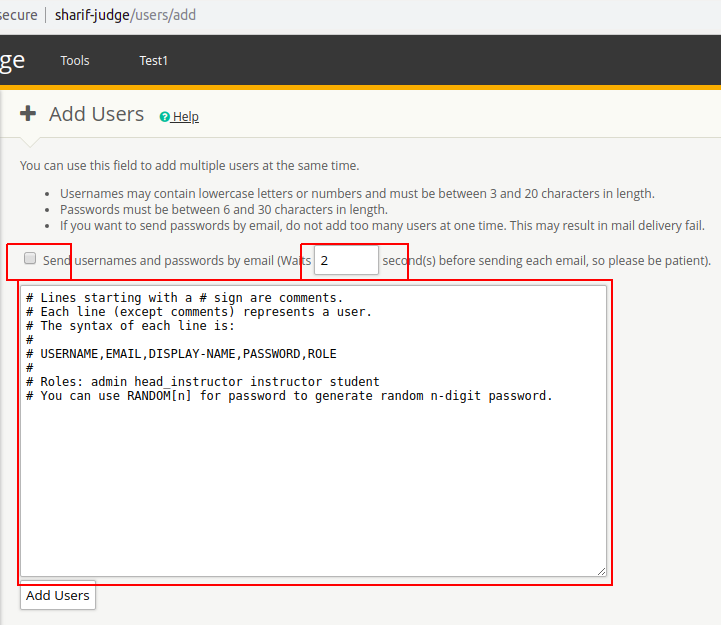
\includegraphics[width=0.5\textwidth]{kepatuhan_1_3_1_add_user}  
		\caption[Kriteria Sukses 1.3.1 - Elemen yang Tidak Diberi Label Pada Halaman \textit{Add Users}]{Kriteria Sukses 1.3.1 - Elemen yang Tidak Diberi Label Pada Halaman \textit{Add Users}} 
		\label{fig:kepatuhan_1_3_1_add_user} 
	\end{figure}
	\item Dalam halaman \textit{Add Assignment} ada elemen dalam form \textit{problems} tidak diberi label. Kesalahan dapat dilihat pada potongan kode \ref{ls_kepatuhan_1_3_1_add_assignment}.
	\begin{lstlisting}[basicstyle=\ttfamily, frame=single,
	columns=fullflexible, keepspaces=true, breaklines=true, label=ls_kepatuhan_1_3_1_add_assignment, caption=Kriteria Sukses 1.3.1 - Elemen Dalam Form yang Tidak Diberi Label]
	...
	<td><input type="text" name="name[]" class="sharif_input short" value="Problem "/></td>\
	...
	\end{lstlisting}
	
	\item Dalam halaman \textit{Problem} terdapat elemen form yang tidak diberi label.
	\begin{figure}[H]
		\centering  
		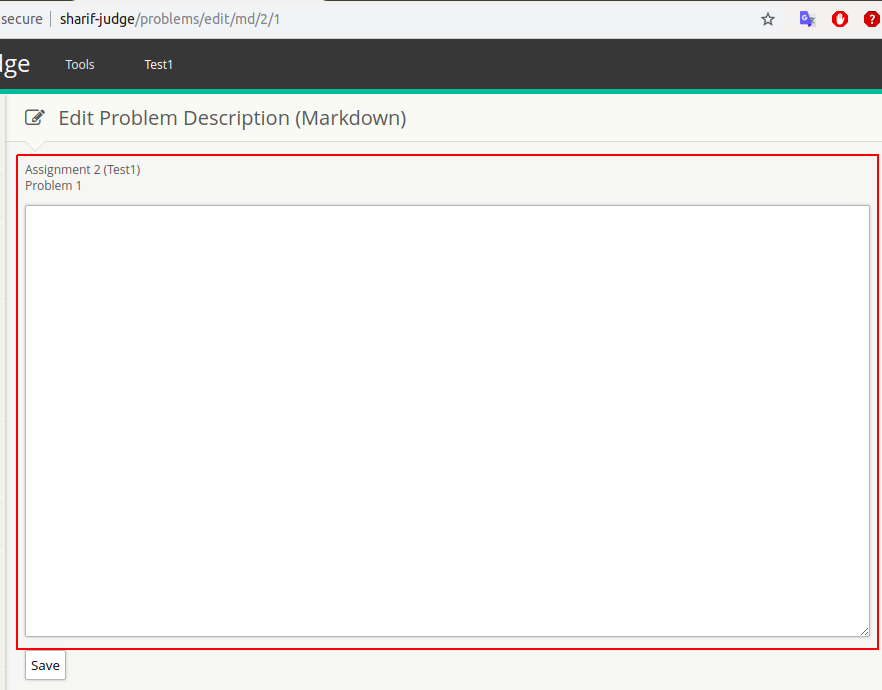
\includegraphics[width=0.5\textwidth]{kepatuhan_1_3_1_problem_edit_markdown}  
		\caption[Kriteria Sukses 1.3.1 - Elemen yang Tidak Diberi Label Pada Halaman \textit{Problems} Bagian \textit{Edit Markdown}]{Kriteria Sukses 1.3.1 - Elemen yang Tidak Diberi Label Pada Halaman \textit{Problems} Bagian \textit{Edit Markdown}} 
		\label{fig:kepatuhan_1_3_1_problem_edit_markdown} 
	\end{figure}
	\begin{figure}[H]
		\centering  
		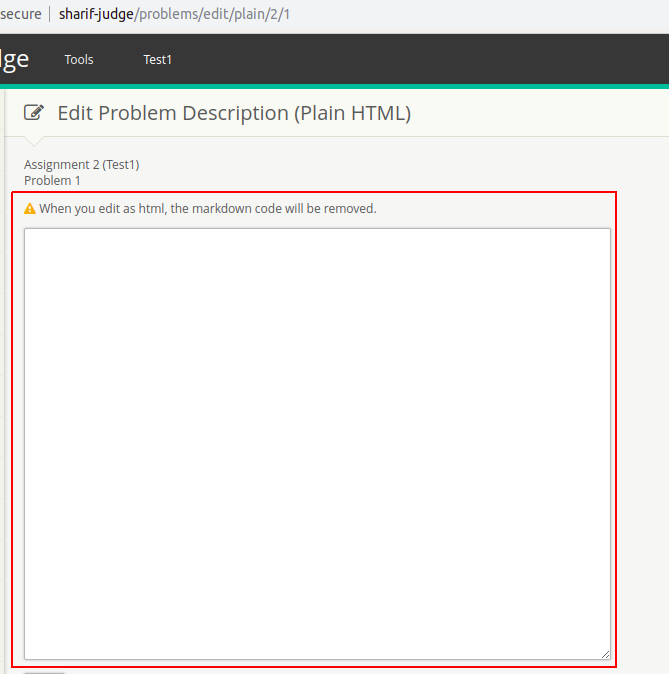
\includegraphics[width=0.5\textwidth]{kepatuhan_1_3_1_edit_plain_html}  
		\caption[Kriteria Sukses 1.3.1 - Elemen yang Tidak Diberi Label Pada Halaman \textit{Problems} Bagian \textit{Edit Plain Html}]{Kriteria Sukses 1.3.1 - Elemen yang Tidak Diberi Label Pada Halaman \textit{Problems} Bagian \textit{Edit Plain Html}} 
		\label{fig:kepatuhan_1_3_1_plain_html} 
	\end{figure}
\end{itemize}

\subsubsection{Kriteria Sukses 1.3.2 Meaningful Sequence}
\label{subsubsec:kepatuhan_kriteria_1.3.2}
(Sukses) \\

Kriteria ini sukses dipatuhi karena setiap halaman pada \textit{SharIF Judge} memiliki urutan baca dan navigasi yang benar.

\subsubsection{Kriteria Sukses 1.3.3 Sensory Characteristics}
\label{subsubsec:kepatuhan_kriteria_1.3.3}
(Sukses)\\

Kriteria ini sukses dipatuhi karena petunjuk yang diberikan pada aplikasi \textit{SharIF Judge} tidak hanya bergantung pada komponen karakteristik sensorik seperti bentuk, warna, ukuran, lokasi visual, orientasi, atau suara.

\subsubsection{Kriteria Sukses 1.3.4 Orientation}
\label{subsubsec:kepatuhan_kriteria_1.3.4}
(Sukses) \\

Kriteria ini sukses dipatuhi karena konten dari \textit{SharIF Judge} dapat ditampilkan dalam orientasi \textit{portrait} atau \textit{landscape}.

\subsubsection{Kriteria Sukses 1.3.5 Identify Input Purpose}
\label{subsubsec:kepatuhan_kriteria_1.3.5}
(Tidak Sukses)\\

Kriteria ini tidak sukses karena masih ada bidang masukan yang tidak memiliki label, salah satunya pada halaman \textit{Problems} bagian \textit{Edit Markdown}. Kesalahan dapat dilihat pada potongan kode \ref{ls_kepatuhan_1_3_5}.
\begin{lstlisting}[basicstyle=\ttfamily, frame=single,
columns=fullflexible, keepspaces=true, breaklines=true, label=ls_kepatuhan_1_3_5, caption=Kriteria Sukses 1.3.5 - Elemen Tidak Diberi Label Pada Halaman \textit{Problems} Bagian \textit{Edit Markdown}]
...
<p class="input_p">
	<textarea name="text">{{ problem.description }}</textarea>
</p>
...
\end{lstlisting}

\subsubsection{Kriteria Sukses 1.3.6 Identify Purpose}
\label{subsubsec:kepatuhan_kriteria_1.3.6}
(Tidak Sukses) \\

Kriteria ini tidak sukses dipatuhi karena ada elemen \textit{HTML} yang seharusnya dapat dipakai tetapi tidak digunakan, seperti bagian navigasi dan judul bagian. Kesalahan dapat dilihat pada potongan kode \ref{ls_kepatuhan_1_3_6}.
\begin{lstlisting}[basicstyle=\ttfamily, frame=single,
columns=fullflexible, keepspaces=true, breaklines=true, label=ls_kepatuhan_1_3_6, caption=Kriteria Sukses 1.3.6 - \textit{Sidebar}]
...
<div id="side_bar" class="sidebar_open">
	<ul>
		<li class="color-dashboard{{ selected=='dashboard' ? ' selected' }}">
...
\end{lstlisting}

\subsubsection{Kriteria Sukses 1.4.1 Use of Color}
\label{subsubsec:kepatuhan_kriteria_1.4.1}
(Sukses) \\

Kriteria ini sukses dipatuhi karena warna tidak digunakan sebagai satu-satunya cara untuk menyampaikan informasi, menunjukkan aksi, menampilkan respon, atau membedakan elemen visual. Selain warna, ada juga teks yang menjelaskan informasi yang ditampilkan.

\subsubsection{Kriteria Sukses 1.4.2 Audio Control}
\label{subsubsec:kepatuhan_kriteria_1.4.2}
(Sukses) \\

Kriteria ini sukses dipatuhi karena pada aplikasi \textit{SharIF Judge} tidak terdapat konten berbasis waktu.

\subsubsection{Kriteria Sukses 1.4.3 Contrast (Minimum)}
\label{subsubsec:kepatuhan_kriteria_1.4.3}
(Tidak Sukses) \\

Kriteria ini tidak sukses dipatuhi karena pada aplikasi \textit{SharIF Judge} terdapat beberapa teks dengan rasio kontras kurang dari 4.5:1, antara lain:
\begin{itemize}
	\item Navigasi Atas: Teks tempat waktu yang tersisa untuk mengumpulkan suatu \textit{Assignment} memiliki rasio kontras 2.52:1 terhadap warna latar belakangnya. Tampilan halaman web dapat dilihat pada gambar \ref{fig:kepatuhan_1_4_3_navigasi_atas}.
	\begin{figure}[H]
		\centering  
		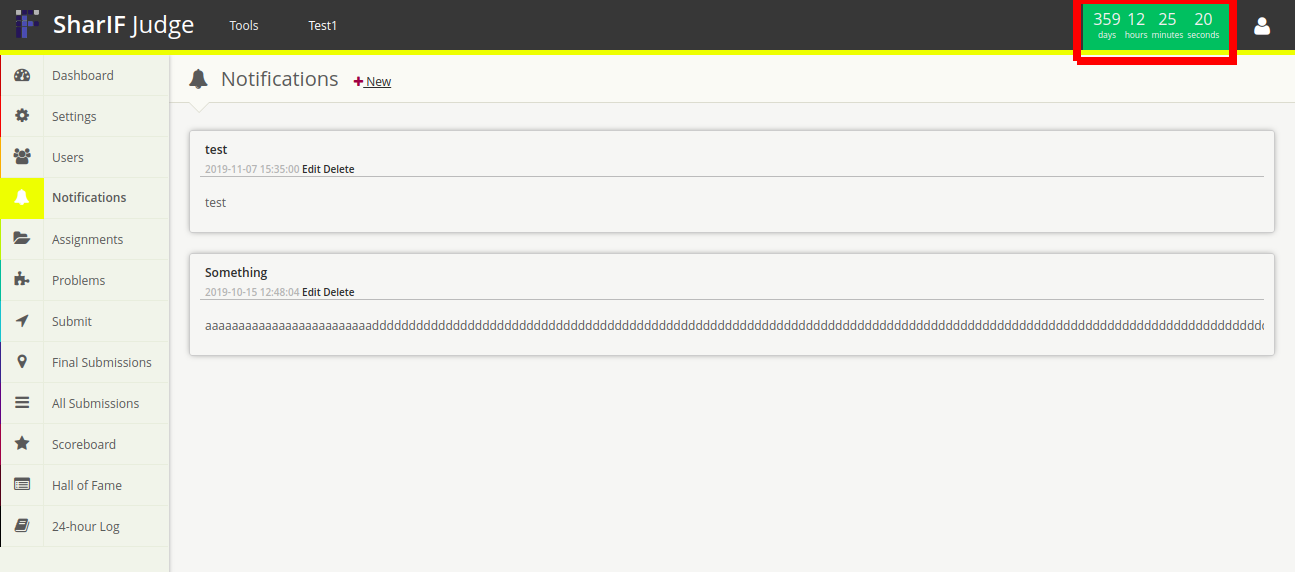
\includegraphics[scale=0.25]{kepatuhan_1_4_3_navigasi_atas}  
		\caption[Kriteria Sukses 1.4.3 - Kontras Elemen Navigasi Atas]{Kriteria Sukses 1.4.3 - Kontras Elemen Navigasi Atas} 
		\label{fig:kepatuhan_1_4_3_navigasi_atas} 
	\end{figure}

	\item Halaman \textit{Dashboard}: Teks pada tombol \textit{today} memiliki rasio kontras 4.01:1 terhadap warna latar belakangnya. Teks pada kalender memiliki rasio kontras 2.69:1 terhadap warna latar belakangnya. Teks pada kalender yang menunjukkan tanggal memiliki rasio kontras 1.57:1 terhadap warna latar belakangnya. Teks yang menunjukkan waktu notifikasi dibuat memiliki rasio kontras 2.07:1 terhadap warna latar belakangnya. Tampilan halaman web dapat dilihat pada gambar \ref{fig:kepatuhan_1_4_3_dashboard}.
	\begin{figure}[H]
		\centering  
		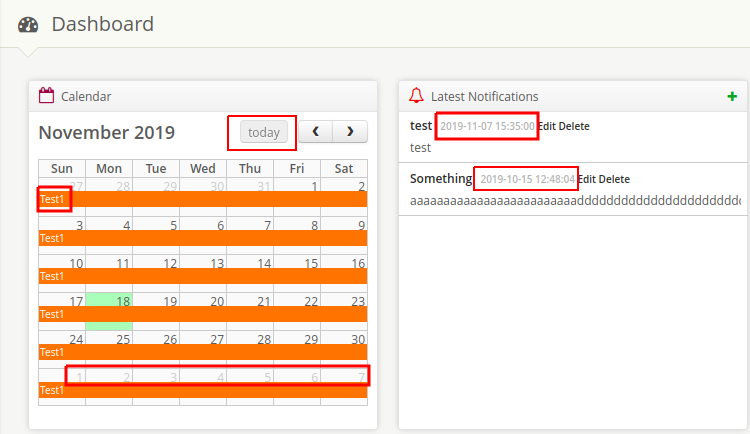
\includegraphics[scale=0.5]{kepatuhan_1_4_3_dashboard}  
		\caption[Kriteria Sukses 1.4.3 - Kontras Elemen Dashboard]{Kriteria Sukses 1.4.3 - Kontras Elemen Dashboard} 
		\label{fig:kepatuhan_1_4_3_dashboard} 
	\end{figure}

	\item Halaman \textit{Settings}: Informasi tambahan pada bidang masukkan memiliki rasio kontras 3.55:1 terhadap warna latar belakangnya. Informasi peringatan pada bidang masukkan memiliki rasio kontras 3.69:1 terhadap warna latar belakangnya. Tampilan halaman web dapat dilihat pada gambar \ref{fig:kepatuhan_1_4_3_settings}.
	\begin{figure}[H]
		\centering  
		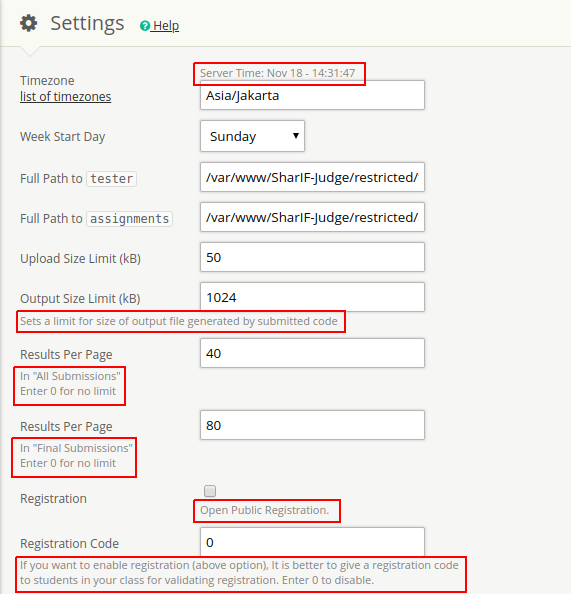
\includegraphics[scale=0.5]{kepatuhan_1_4_3_settings}  
		\caption[Kriteria Sukses 1.4.3 - Kontras Elemen Settings]{Kriteria Sukses 1.4.3 - Kontras Elemen Settings} 
		\label{fig:kepatuhan_1_4_3_settings} 
	\end{figure}

	\item Halaman \textit{Notifications}: Teks yang menunjukkan waktu notifikasi dibuat memiliki rasio kontras 1.91:1 terhadap warna latar belakangnya. Tampilan halaman web dapat dilihat pada gambar \ref{fig:kepatuhan_1_4_3_notifications}.
	\begin{figure}[H]
		\centering  
		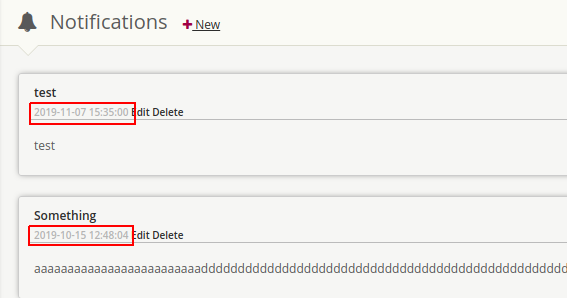
\includegraphics[scale=0.5]{kepatuhan_1_4_3_notifications}  
		\caption[Kriteria Sukses 1.4.3 - Kontras Elemen Notifications]{Kriteria Sukses 1.4.3 - Kontras Elemen Notifications} 
		\label{fig:kepatuhan_1_4_3_notifications} 
	\end{figure}
	
	\item Halaman \textit{Assignment}: Teks yang berwana merah pada tabel \textit{Assignment} memiliki rasio kontras 3.89:1 terhadap warna latar belakangnya. Tampilan halaman web dapat dilihat pada gambar \ref{fig:kepatuhan_1_4_3_assignments}.
	\begin{figure}[H]
		\centering  
		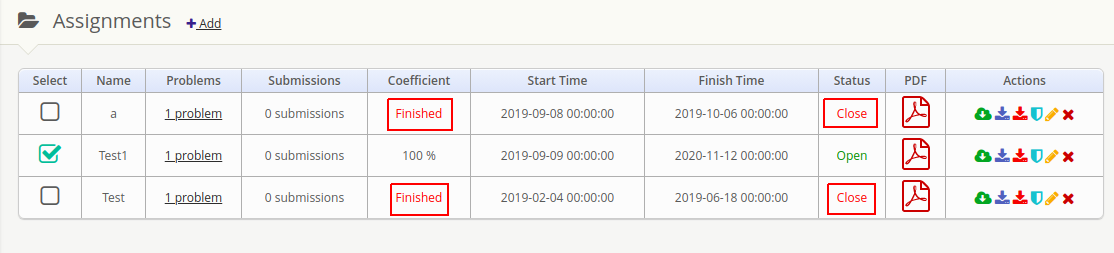
\includegraphics[scale=0.3]{kepatuhan_1_4_3_assignments}  
		\caption[Kriteria Sukses 1.4.3 - Kontras Elemen Assignments]{Kriteria Sukses 1.4.3 - Kontras Elemen Assignments} 
		\label{fig:kepatuhan_1_4_3_assignments} 
	\end{figure}
	
	\item Halaman \textit{Add Assignment}: Informasi tambahan pada bidang masukkan memiliki rasio kontras 3.55:1 terhadap warna latar belakangnya. Informasi peringatan pada bidang masukkan memiliki rasio kontras 3.69:1 terhadap warna latar belakangnya. Tampilan halaman web dapat dilihat pada gambar \ref{fig:kepatuhan_1_4_3_add_assignment}.
	\begin{figure}[H]
		\centering  
		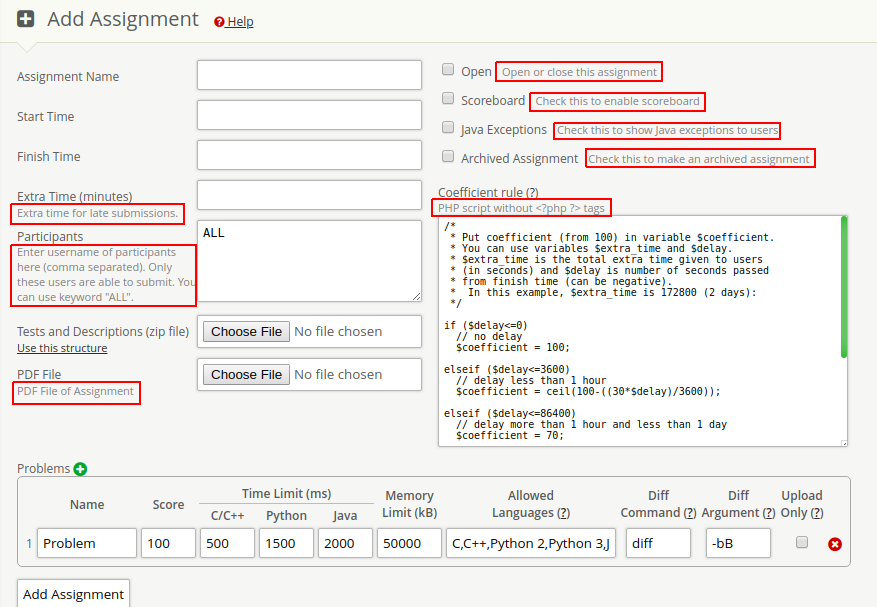
\includegraphics[scale=0.5]{kepatuhan_1_4_3_add_assignment}  
		\caption[Kriteria Sukses 1.4.3 - Kontras Elemen \textit{Add Assignments}]{Kriteria Sukses 1.4.3 - Kontras Elemen \textit{Add Assignments}} 
		\label{fig:kepatuhan_1_4_3_add_assignment} 
	\end{figure}
	
\end{itemize}

\subsubsection{Kriteria Sukses 1.4.4 Resize text}
\label{subsubsec:kepatuhan_kriteria_1.4.4}
(Tidak Sukses) \\

Kriteria ini tidak sukses dipatuhi karena fungsionalitas \textit{navigation bar} tidak berjalan pada pembesaran 125 persen. Tampilan halaman web dapat dilihat pada gambar \ref{fig:kepatuhan_1_4_4_nav_bar}.
\begin{figure}[H]
	\centering  
	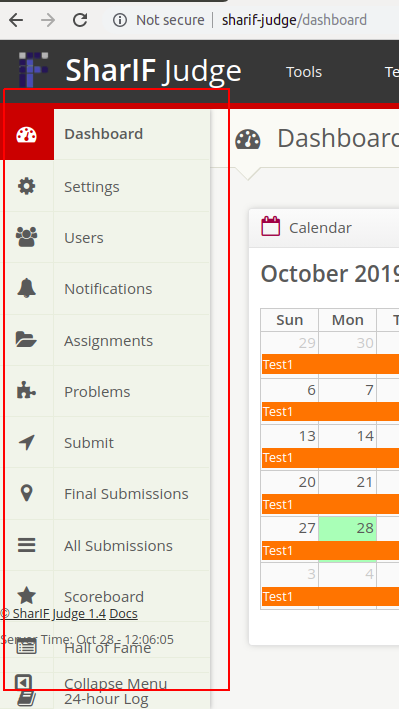
\includegraphics[width=0.5\textwidth]{kepatuhan_1_4_4_nav_bar}  
	\caption[Kriteria Sukses 1.4.4 - Sidenav]{Kriteria Sukses 1.4.4 - Sidenav} 
	\label{fig:kepatuhan_1_4_4_nav_bar} 
\end{figure}


\subsubsection{Kriteria Sukses 1.4.5 Images of Text}
\label{subsubsec:kepatuhan_kriteria_1.4.5}
(Sukses) \\

Kriteria ini sukses dipatuhi karena semua gambar teks yang ada pada aplikasi \textit{SharIF Judge} penting untuk informasi yang disampaikan.

\subsubsection{Kriteria Sukses 1.4.6 Contrast (Enhanced)}
\label{subsubsec:kepatuhan_kriteria_1.4.6}

(Tidak Sukses) \\

Kriteria ini tidak sukses dipatuhi karena pada aplikasi \textit{SharIF Judge} terdapat beberapa teks dengan rasio kontras kurang dari 4.5:1, antara lain:
\begin{itemize}
	\item Navigasi Atas: Teks tempat waktu yang tersisa untuk mengumpulkan suatu \textit{Assignment} memiliki rasio kontras 2.52:1 terhadap warna latar belakangnya. Tampilan halaman web dapat dilihat pada gambar \ref{fig:kepatuhan_1_4_6_navigasi_atas}.
	\begin{figure}[H]
		\centering  
		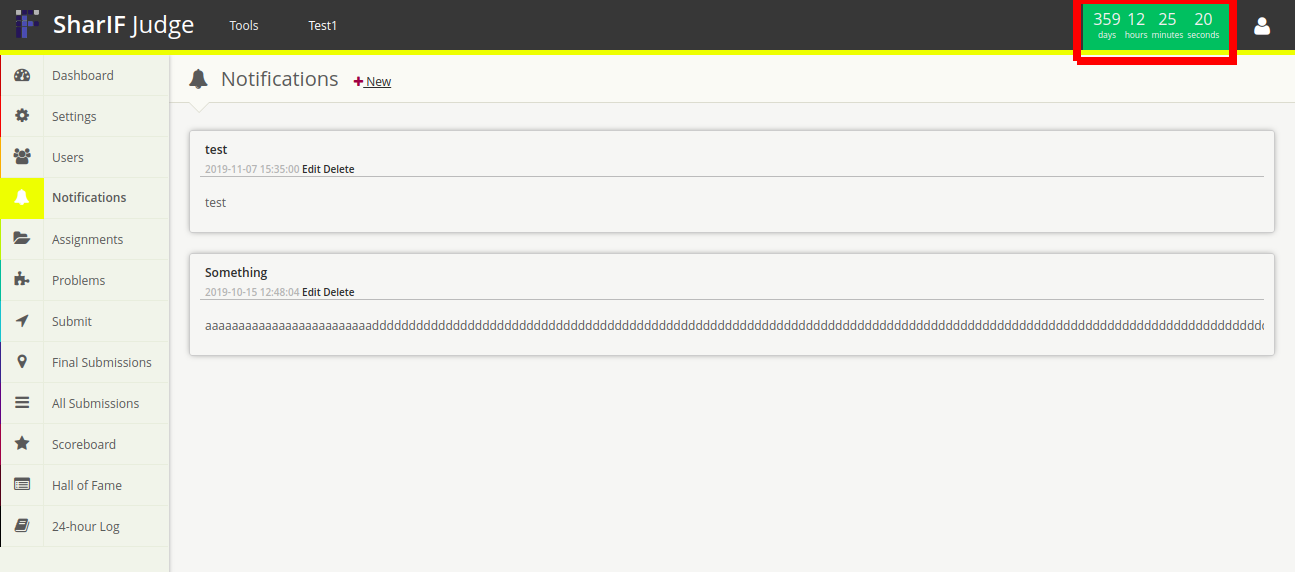
\includegraphics[scale=0.25]{kepatuhan_1_4_6_navigasi_atas}  
		\caption[Kriteria Sukses 1.4.6 - Kontras Elemen Navigasi Atas]{Kriteria Sukses 1.4.6 - Kontras Elemen Navigasi Atas} 
		\label{fig:kepatuhan_1_4_6_navigasi_atas} 
	\end{figure}

	\item Halaman \textit{Dashboard}: Teks pada tombol \textit{today} memiliki rasio kontras 4.01:1 terhadap warna latar belakangnya. Teks pada kalender memiliki rasio kontras 2.69:1 terhadap warna latar belakangnya. Teks pada kalender yang menunjukkan tanggal memiliki rasio kontras 1.57:1 terhadap warna latar belakangnya. Teks yang menunjukkan waktu notifikasi dibuat memiliki rasio kontras 2.07:1 terhadap warna latar belakangnya. Tampilan halaman web dapat dilihat pada gambar \ref{fig:kepatuhan_1_4_6_dashboard}.
	\begin{figure}[H]
		\centering  
		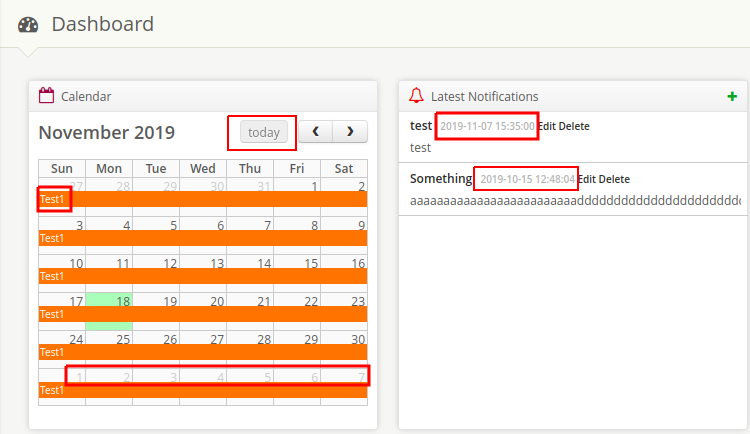
\includegraphics[scale=0.5]{kepatuhan_1_4_6_dashboard}  
		\caption[Kriteria Sukses 1.4.6 - Kontras Elemen Dashboard]{Kriteria Sukses 1.4.6 - Kontras Elemen Dashboard} 
		\label{fig:kepatuhan_1_4_6_dashboard} 
	\end{figure}

	\item Halaman \textit{Settings}: Informasi tambahan pada bidang masukkan memiliki rasio kontras 3.55:1 terhadap warna latar belakangnya. Informasi peringatan pada bidang masukkan memiliki rasio kontras 3.69:1 terhadap warna latar belakangnya. Tampilan halaman web dapat dilihat pada gambar \ref{fig:kepatuhan_1_4_6_settings}.
	\begin{figure}[H]
		\centering  
		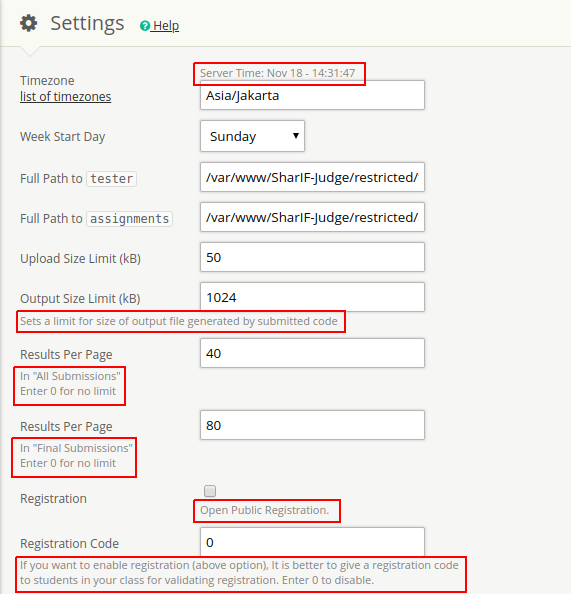
\includegraphics[scale=0.5]{kepatuhan_1_4_6_settings}  
		\caption[Kriteria Sukses 1.4.6 - Kontras Elemen Settings]{Kriteria Sukses 1.4.6 - Kontras Elemen Settings} 
		\label{fig:kepatuhan_1_4_6_settings} 
	\end{figure}

	\item Halaman \textit{Notifications}: Teks yang menunjukkan waktu notifikasi dibuat memiliki rasio kontras 1.91:1 terhadap warna latar belakangnya. Tampilan halaman web dapat dilihat pada gambar \ref{fig:kepatuhan_1_4_6_notifications}.
	\begin{figure}[H]
		\centering  
		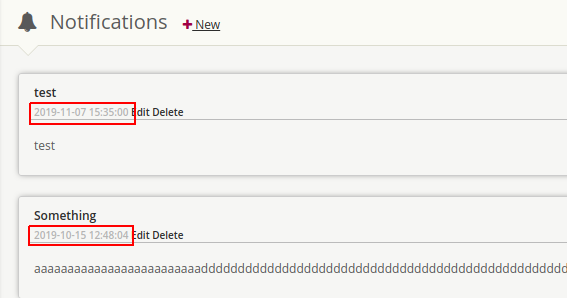
\includegraphics[scale=0.5]{kepatuhan_1_4_6_notifications}  
		\caption[Kriteria Sukses 1.4.6 - Kontras Elemen Notifications]{Kriteria Sukses 1.4.6 - Kontras Elemen Notifications} 
		\label{fig:kepatuhan_1_4_6_notifications} 
	\end{figure}

	\item Halaman \textit{Assignment}: Teks yang berwana merah pada tabel \textit{Assignment} memiliki rasio kontras 3.89:1 terhadap warna latar belakangnya. Tampilan halaman web dapat dilihat pada gambar \ref{fig:kepatuhan_1_4_6_assignments}.
	\begin{figure}[H]
		\centering  
		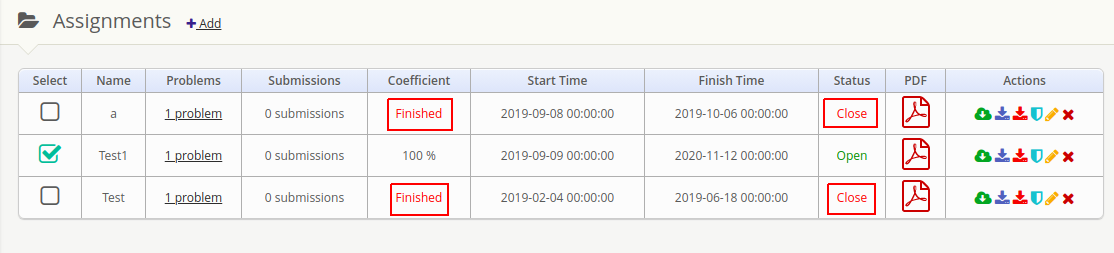
\includegraphics[scale=0.3]{kepatuhan_1_4_6_assignments}  
		\caption[Kriteria Sukses 1.4.6 - Kontras Elemen Assignments]{Kriteria Sukses 1.4.6 - Kontras Elemen Assignments} 
		\label{fig:kepatuhan_1_4_6_assignments} 
	\end{figure}

	\item Halaman \textit{Add Assignment}: Informasi tambahan pada bidang masukkan memiliki rasio kontras 3.55:1 terhadap warna latar belakangnya. Informasi peringatan pada bidang masukkan memiliki rasio kontras 3.69:1 terhadap warna latar belakangnya. Tampilan halaman web dapat dilihat pada gambar \ref{fig:kepatuhan_1_4_6_add_assignment}.
	\begin{figure}[H]
		\centering  
		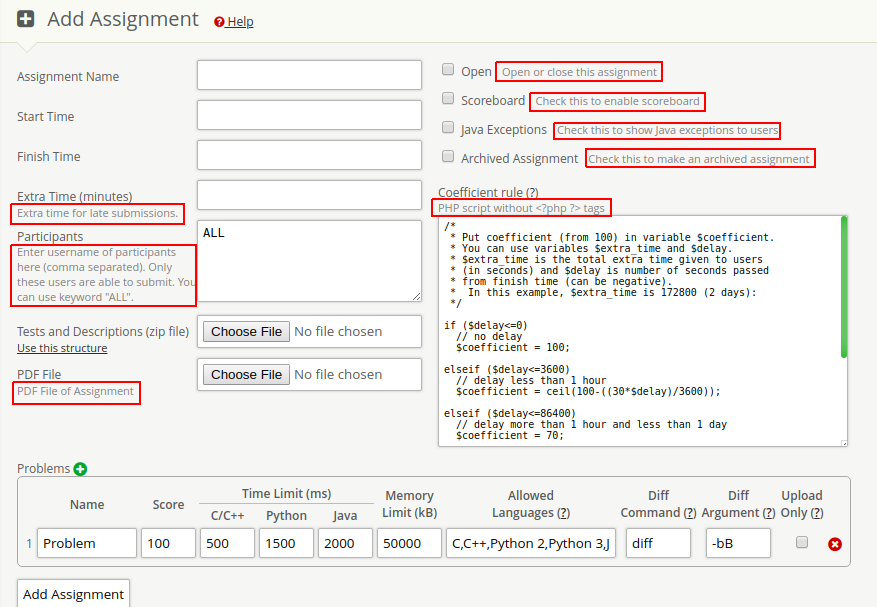
\includegraphics[scale=0.5]{kepatuhan_1_4_6_add_assignment}  
		\caption[Kriteria Sukses 1.4.6 - Kontras Elemen Add Assignments]{Kriteria Sukses 1.4.6 - Kontras Elemen Add Assignments} 
		\label{fig:kepatuhan_1_4_6_add_assignment} 
	\end{figure}

\end{itemize}

\subsubsection{Kriteria Sukses 1.4.7 Low atau No Background Audio}
\label{subsubsec:kepatuhan_kriteria_1.4.7}
(Sukses) \\

Kriteria ini sukses dipatuhi karena pada aplikasi \textit{SharIF Judge} tidak terdapat konten berbasis waktu.


\subsubsection{Kriteria Sukses 1.4.8 Visual Presentation}
\label{subsubsec:kepatuhan_kriteria_1.4.8}
(Tidak Sukses) \\

Kriteria ini tidak sukses dipatuhi karena pada halaman \textit{Dashboard} dan \textit{Notifications} teks yang menampilkan isi notifikasi memiliki lebar lebih dari 80 karakter. Tampilan halaman web ditampilkan pada gambar \ref{fig:kepatuhan_1_4_8_notifications}.
\begin{figure}[H]
	\centering  
	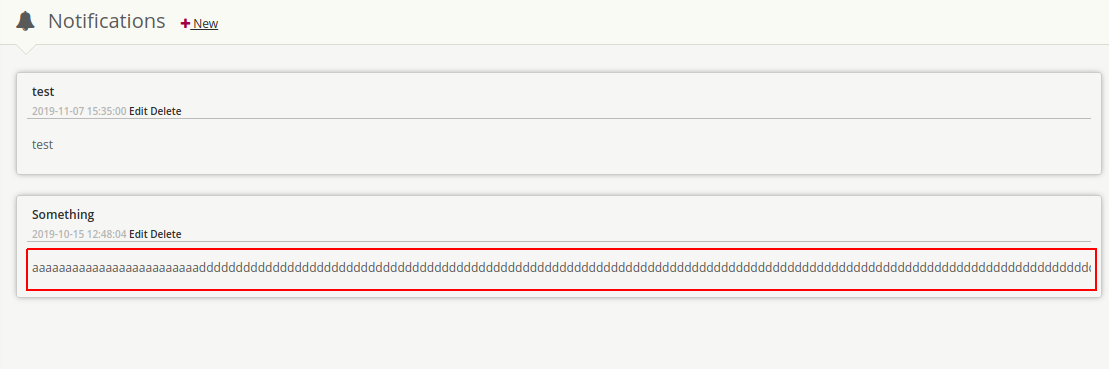
\includegraphics[scale=0.25]{kepatuhan_1_4_8_notifications}  
	\caption[Kriteria Sukses 1.4.8 - Notifications]{Kriteria Sukses 1.4.8 - Notifications} 
	\label{fig:kepatuhan_1_4_8_notifications} 
\end{figure}

\subsubsection{Kriteria Sukses 1.4.9 Images of Text (No Exception)}
\label{subsubsec:kepatuhan_kriteria_1.4.9}
(Sukses) \\

Kriteria ini sukses dipatuhi karena semua gambar teks yang ada pada aplikasi \textit{SharIF Judge} penting untuk informasi yang disampaikan.

\subsubsection{Kriteria Sukses 1.4.10 Reflow}
\label{subsubsec:kepatuhan_kriteria_1.4.10}
(Tidak Sukses) \\

Kriteria ini tidak sukses dipatuhi karena pada setiap halaman aplikasi \textit{SharIF Judge} memerlukan \textit{scroll} secara horizontal ketika ditampilkan pada resolusi layar 1280 pixel dengan pembesaran 400 persen. Tampilan halaman web dapat dilihat pada gambar \ref{fig:kepatuhan_1_4_10_reflow}
\begin{figure}[H]
	\centering  
	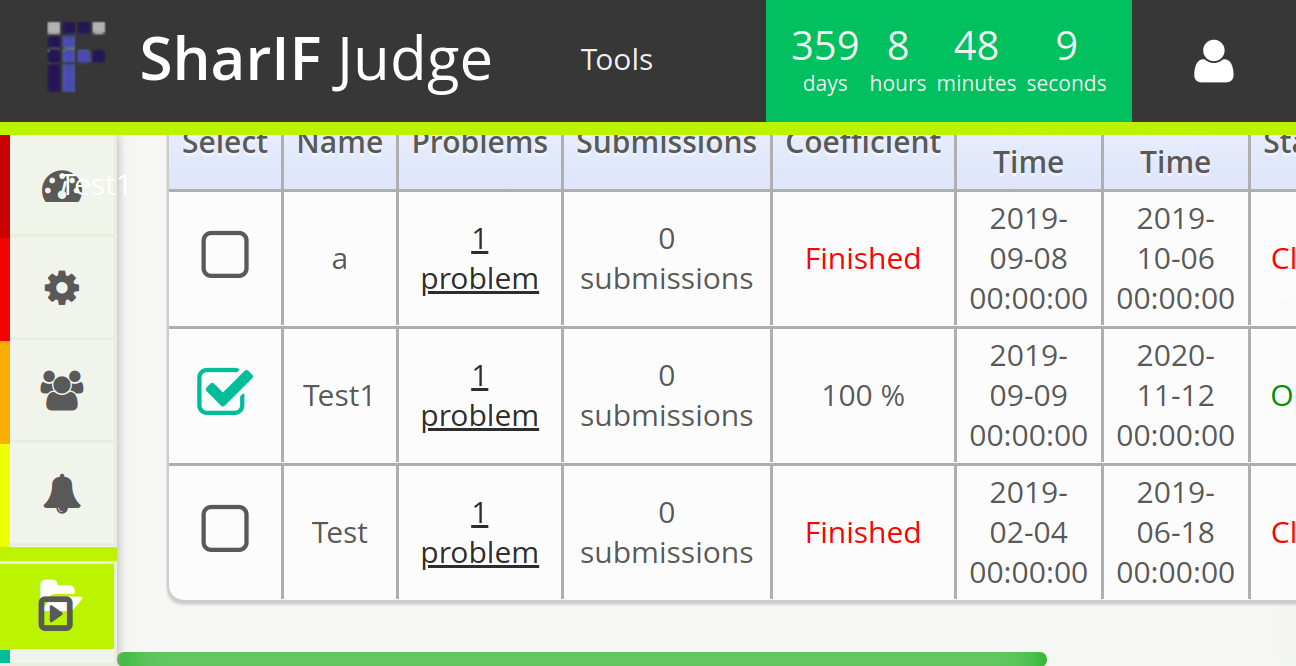
\includegraphics[scale=0.25]{kepatuhan_1_4_10}  
	\caption[Kriteria Sukses 1.4.10 - Horizontal \textit{Scroll}]{Kriteria Sukses 1.4.10 - Horizontal \textit{Scroll}} 
	\label{fig:kepatuhan_1_4_10_reflow} 
\end{figure}

\subsubsection{Kriteria Sukses 1.4.11 Non-text Contrast}
\label{subsubsec:kepatuhan_kriteria_1.4.11}
(Diabaikan) \\

Kriteria ini diabaikan karena pengukuran kontras sulit untuk dilakukan. Tampilan halaman web dapat dilihat pada gambar \ref{fig:kepatuhan_1_4_11_reflow}.
\begin{figure}[H]
	\centering  
	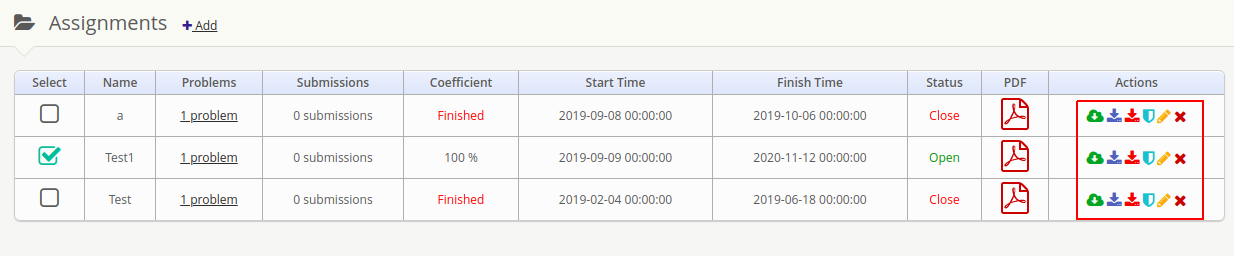
\includegraphics[scale=0.3]{kepatuhan_1_4_11}  
	\caption[Kriteria Sukses 1.4.11 - Ikon Pada Halaman \textit{Assignments}]{Kriteria Sukses 1.4.11 - Ikon Pada Halaman \textit{Assignments}} 
	\label{fig:kepatuhan_1_4_11_reflow} 
\end{figure}

\subsubsection{Kriteria Sukses 1.4.12 Text Spacing}
\label{subsubsec:kepatuhan_kriteria_1.4.12}

\subsubsection{Kriteria Sukses 1.4.13 Content on Hover or Focus}
\label{subsubsec:kepatuhan_kriteria_1.4.13}
(Sukses) \\

Kriteria ini sukses dipatuhi karena setiap konten tambahan yang muncul sesaat ketika suatu elemen menerima penunjuk kursor atau fokus \textit{keyboard}, konten tambahan tersebut dapat disingkirkan, dapat ditunjuk, dan persisten.

\subsection{\textit{Operable}}
\label{subsec:kepatuhan_operable}

\subsubsection{Kriteria Sukses 2.1.1 Keyboard}
\label{subsubsec:kepatuhan_kriteria_2.1.1}
(Tidak Sukses) \\

Kriteria ini tidak sukses dipatuhi karena :
\begin{itemize}
	\item Tombol \textit{Collapse Menu} pada \textit{sidebar} tidak dapat dioperasikan dengan keyboard. Tampilan halaman web dapat dilihat pada gambar \ref{fig:kepatuhan_2_1_1_collapse_menu}.
	\begin{figure}[H]
		\centering  
		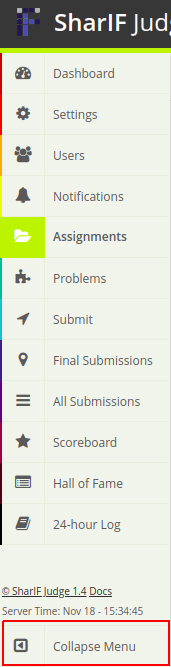
\includegraphics[scale=0.5]{kepatuhan_2_1_1_collapse_menu}  
		\caption[Kriteria Sukses 2.1.1 - \textit{Collapse Menu}]{Kriteria Sukses 2.1.1 - \textit{Collapse Menu}} 
		\label{fig:kepatuhan_2_1_1_collapse_menu} 
	\end{figure}

	\item Tombol \textit{Tools} pada \textit{Menu} tidak dapat dioperasikan dengan keyboard. Tampilan halaman web dapat dilihat pada gambar \ref{fig:kepatuhan_2_1_1_tools}.
	\begin{figure}[H]
		\centering  
		
\includegraphics[scale=0.5]{kepatuhan_2_1_1_tools}  
		\caption[Kriteria Sukses 2.1.1 - \textit{Tools}]{Kriteria Sukses 2.1.1 - \textit{Tools}} 
		\label{fig:kepatuhan_2_1_1_tools} 
	\end{figure}

\end{itemize}

\subsubsection{Kriteria Sukses 2.1.2 No Keyboard Trap}
\label{subsubsec:kepatuhan_kriteria_2.1.2}
(Tidak Sukses) \\

Kriteria ini tidak sukses dipatuhi karena :
\begin{itemize}
	\item Dalam halaman \textit{Settings} ada \textit{input field} yang fokusnya tidak dapat dipindahkan menggunakan antarmuka \textit{keyboard}. \textit{Input field} yang dimaksud dapat dilihat pada gambar \ref{fig:kepatuhan_2_1_2_settings}.
	\begin{figure}[H]
		\centering  
		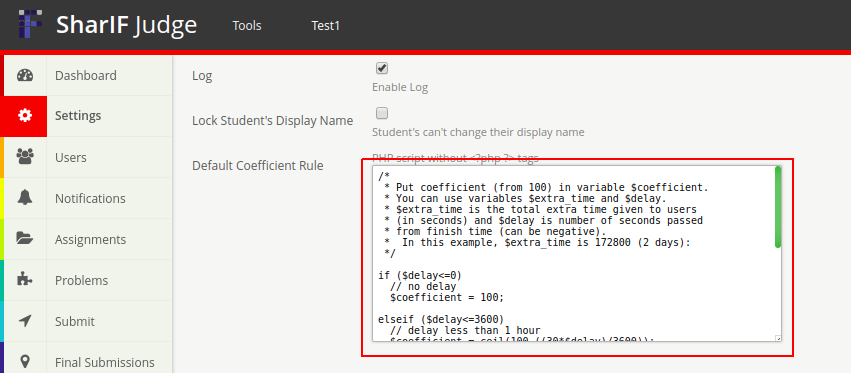
\includegraphics[scale=0.5]{kepatuhan_2_1_2_settings}  
		\caption[Kriteria Sukses 2.1.2 - \textit{Settings}]{Kriteria Sukses 2.1.2 - \textit{Settings}} 
		\label{fig:kepatuhan_2_1_2_settings} 
	\end{figure}

	\item Dalam halaman \textit{Add User} ada \textit{input field} yang fokusnya tidak dapat dipindahkan menggunakan antarmuka \textit{keyboard}.\textit{Input field} yang dimaksud dapat dilihat pada gambar \ref{fig:kepatuhan_2_1_2_add_user}.
	\begin{figure}[H]
		\centering  
		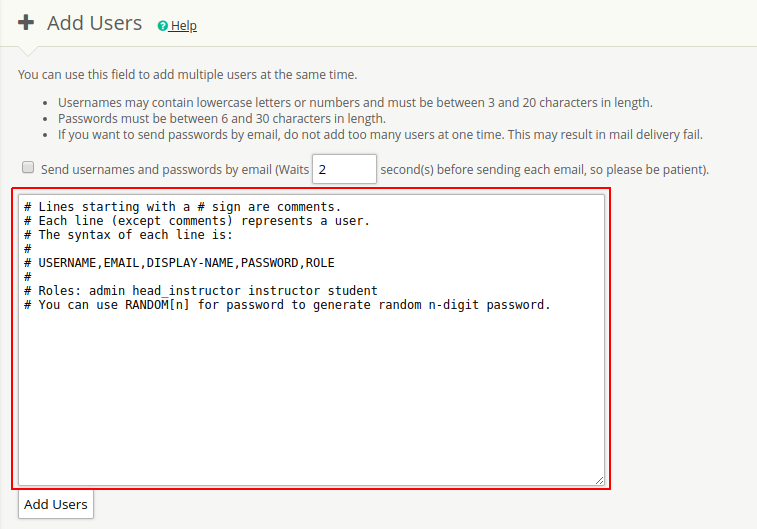
\includegraphics[scale=0.5]{kepatuhan_2_1_2_add_user}  
		\caption[Kriteria Sukses 2.1.2 - \textit{Add User}]{Kriteria Sukses 2.1.2 - \textit{Add User}} 
		\label{fig:kepatuhan_2_1_2_add_user} 
	\end{figure}

	\item Dalam halaman \textit{Add Assignment} ada \textit{input field} yang fokusnya tidak dapat dipindahkan menggunakan antarmuka \textit{keyboard}.\textit{Input field} yang dimaksud dapat dilihat pada gambar \ref{fig:kepatuhan_2_1_2_add_assignment}.
	\begin{figure}[H]
		\centering  
		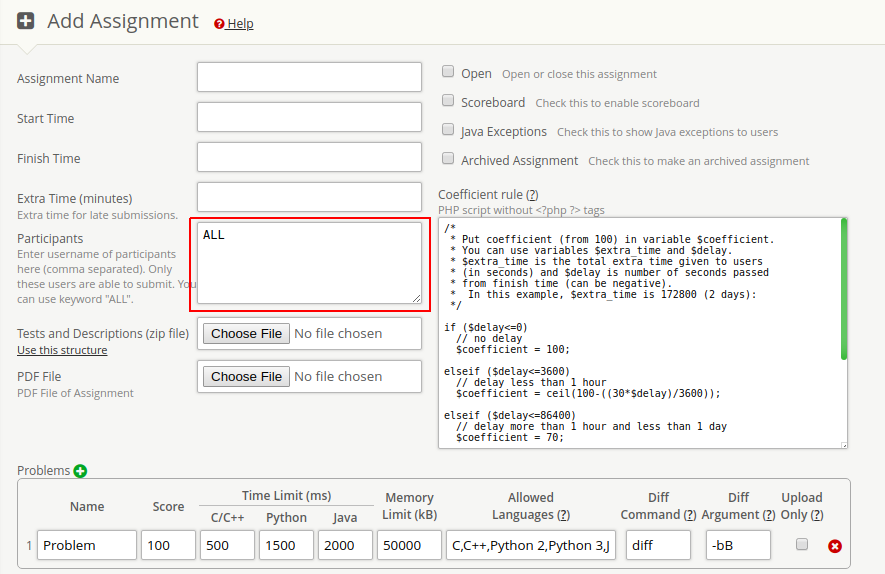
\includegraphics[scale=0.5]{kepatuhan_2_1_2_add_assignment}  
		\caption[Kriteria Sukses 2.1.2 - \textit{Add Assignment}]{Kriteria Sukses 2.1.2 - \textit{Add Assignment}} 
		\label{fig:kepatuhan_2_1_2_add_assignment} 
	\end{figure}

	\item Dalam halaman \textit{Problems}(\textit{Edit Markdown}) ada \textit{input field} yang fokusnya tidak dapat dipindahkan menggunakan antarmuka \textit{keyboard}.\textit{Input field} yang dimaksud dapat dilihat pada gambar \ref{fig:kepatuhan_2_1_2_problems_edit_markdown}.
	\begin{figure}[H]
		\centering  
		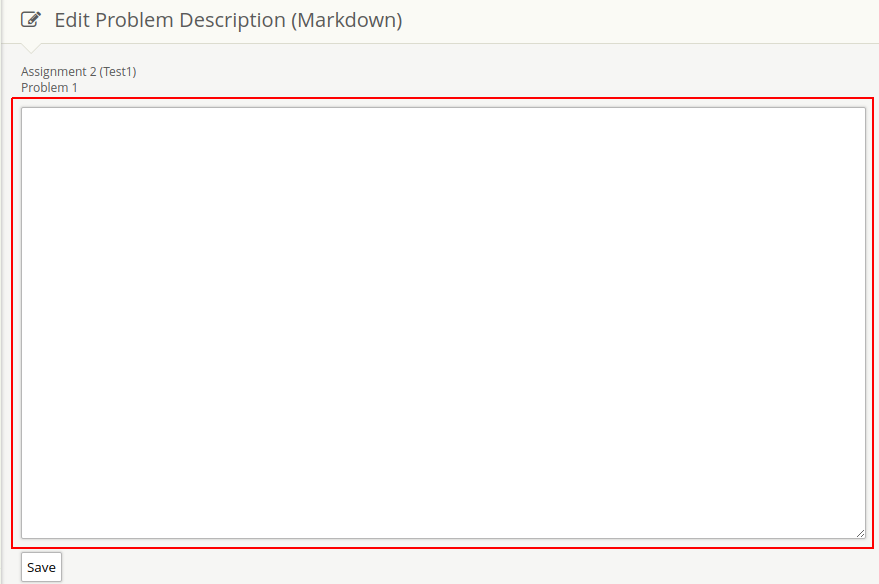
\includegraphics[scale=0.5]{kepatuhan_2_1_2_problems_edit_markdown}  
		\caption[Kriteria Sukses 2.1.2 - \textit{Problems} Bagian \textit{Edit Markdown}]{Kriteria Sukses 2.1.2 - \textit{Problems} Bagian \textit{Edit Markdown}} 
		\label{fig:kepatuhan_2_1_2_problems_edit_markdown} 
	\end{figure}

\end{itemize}

\subsubsection{Kriteria Sukses 2.1.3 Keyboard (No Exception)}
\label{subsubsec:kepatuhan_kriteria_2.1.3}
(Tidak Sukses) \\

Kriteria ini tidak sukses dipatuhi karena :
\begin{itemize}
	\item Tombol \textit{Collapse Menu} pada \textit{sidebar} tidak dapat dioperasikan dengan keyboard. Tampilan halaman web dapat dilihat pada gambar \ref{fig:kepatuhan_2_1_3_collapse_menu}.
	\begin{figure}[H]
		\centering  
		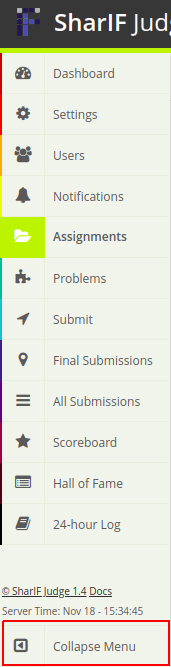
\includegraphics[scale=0.5]{kepatuhan_2_1_3_collapse_menu}  
		\caption[Kriteria Sukses 2.1.3 - \textit{Collapse Menu}]{Kriteria Sukses 2.1.3 - \textit{Collapse Menu}} 
		\label{fig:kepatuhan_2_1_3_collapse_menu} 
	\end{figure}

	\item Tombol \textit{Tools} dan \textit{Assignments} pada \textit{Menu} tidak dapat dioperasikan dengan keyboard. Tampilan halaman web dapat dilihat pada gambar \ref{fig:kepatuhan_2_1_3_tools}.
	\begin{figure}[H]
		\centering  
		
\includegraphics[scale=0.5]{kepatuhan_2_1_3_tools}  
		\caption[Kriteria Sukses 2.1.3 - \textit{Tools}]{Kriteria Sukses 2.1.3 - \textit{Tools}} 
		\label{fig:kepatuhan_2_1_3_tools} 
	\end{figure}

\end{itemize}

\subsubsection{Kriteria Sukses 2.1.4 Character Key Shortcuts}
\label{subsubsec:kepatuhan_kriteria_2.1.4}
(Sukses) \\

Kriteria ini sukses dipatuhi karena pada aplikasi \textit{SharIF Judge} tidak terdapat pintasan \textit{keyboard} untuk konten yang ditampilkan.

\subsubsection{Kriteria Sukses 2.2.1 Timing Adjustable}
\label{subsubsec:kepatuhan_kriteria_2.2.1}
(Sukses) \\

Kriteria ini sukses dipatuhi karena pada aplikasi \textit{SharIF Judge} batas waktu untuk mengumpulkan \textit{Assignment} merupakan hal yang esensial dan perpanjangan batas waktu menyalahi inti dari kegiatan tersebut.

\subsubsection{Kriteria Sukses 2.2.2 Pause, Stop, Hide}
\label{subsubsec:kepatuhan_kriteria_2.2.2}
(Sukses) \\

Kriteria ini sukses dipatuhi karena pada aplikasi \textit{SharIF Judge} satu-satunya informasi yang diperbarui secara otomatis adalah batas waktu pengumpulan \textit{Assignment} yang merupakan bagian dari aktivitas yang esensial.

\subsubsection{Kriteria Sukses 2.2.3 No Timing}
\label{subsubsec:kepatuhan_kriteria_2.2.3}
(Sukses) \\

Kriteria ini sukses dipatuhi karena pada aplikasi \textit{SharIF Judge} waktu pengumpulan \textit{Assignment} bukanlah bagian esensial, pengguna dapat mendapatkan nilai yang sama selama mengumpulkan \textit{Assignment} dalam batas waktu yang telah ditentukan.

\subsubsection{Kriteria Sukses 2.2.4 Interruptions}
\label{subsubsec:kepatuhan_kriteria_2.2.4}
(Sukses) \\

Kriteria ini sukses dipatuhi karena pada aplikasi \textit{SharIF Judge} tidak ada interupsi.

\subsubsection{Kriteria Sukses 2.2.5 Re-authenticating}
\label{subsubsec:kepatuhan_kriteria_2.2.5}
(Tidak Sukses) \\

Kriteria ini tidak sukses dipatuhi karena pada aplikasi \textit{SharIF Judge} ketika sesi autentikasi berakhir, data yang belum disimpan akan hilang.

\subsubsection{Kriteria Sukses 2.2.6 Timeouts}
\label{subsubsec:kepatuhan_kriteria_2.2.6}
(Tidak Sukses) \\

Kriteria ini tidak sukses dipatuhi karena pada aplikasi \textit{SharIF Judge} waktu ketidakaktifan yang dapat menyebabkan kehilangan data kurang dari 20 jam. Pada potongan kode \ref{ls_kepatuhan_2_2_6} ditunjukkan bahwa sesi autentikasi hanya berlangsung selama 2 jam ketika user tidak melakukan tindakan apa pun.
\begin{lstlisting}[basicstyle=\ttfamily, frame=single,
columns=fullflexible, keepspaces=true, breaklines=true, label=ls_kepatuhan_2_2_6, caption=Kriteria Sukses 2.2.6 - Sesi Autentikasi]
...
$config['sess_cookie_name']		= 'shjsession';
$config['sess_expiration']		= 7200;
...
\end{lstlisting}

\subsubsection{Kriteria Sukses 2.3.1 Three Flashes or Below Threshold}
\label{subsubsec:kepatuhan_kriteria_2.3.1}
(Sukses)\\

Kriteria ini sukses dipatuhi karena pada aplikasi \textit{SharIF Judge} tidak ada konten yang berkedip lebih dari tiga detik dalam periode satu detik.

\subsubsection{Kriteria Sukses 2.3.2 Three Flashes}
\label{subsubsec:kepatuhan_kriteria_2.3.2}
(Sukses) \\

Kriteria ini sukses dipatuhi karena pada aplikasi \textit{SharIF Judge} tidak ada konten yang berkedip lebih dari tiga detik dalam periode satu detik.

\subsubsection{Kriteria Sukses 2.3.3 Animation from Interactions}
\label{subsubsec:kepatuhan_kriteria_2.3.3}
(Sukses) \\

Kriteria ini sukses dipatuhi karena satu-satunya animasi yang terdapat di aplikasi \textit{SharIF Judge} adalah tampilan batas waktu pengumpulan \textit{Assignment}, animasi ini penting untuk informasi yang disampaikan.

\subsubsection{Kriteria Sukses 2.4.1 Bypass Blocks}
\label{subsubsec:kepatuhan_kriteria_2.4.1}
(Tidak Sukses) \\

Kriteria ini tidak sukses dipatuhi karena tidak ada mekanisme untuk meloncati menu pada \textit{sidebar}.

\subsubsection{Kriteria Sukses 2.4.2 Page Titled}
\label{subsubsec:kepatuhan_kriteria_2.4.2}
(Sukses) \\

Kriteria ini sukses dipatuhi karena semua halaman pada aplikasi \textit{SharIF Judge} memiliki judul yang menggambarkan topik atau tujuan.

\subsubsection{Kriteria Sukses 2.4.3 Focus Order}
\label{subsubsec:kepatuhan_kriteria_2.4.3}
(Sukses) \\

Kriteria ini sukses dipatuhi karena semua halaman pada aplikasi \textit{SharIF Judge} yang memiliki urutan navigasi dapat menerima fokus dalam urutan yang menjaga makna dan pengoperasiannya.

\subsubsection{Kriteria Sukses 2.4.4 Link Purpose (In Context)}
\label{subsubsec:kepatuhan_kriteria_2.4.4}
(Tidak Sukses) \\

Kriteria ini tidak sukses dipatuhi karena :
\begin{itemize}
	\item Pada halaman \textit{Assignment} ada gambar yang memiliki tautan tetapi tidak ada teks yang menjelaskan tujuan dari tautan tersebut. Pada potongan kode \ref{ls_kepatuhan_2_4_4_assignment} ditunjukkan bahwa gambar pdf memiliki tautan yang tidak memiliki teks yang menjelaskan tujuannya.
	\begin{lstlisting}[basicstyle=\ttfamily, frame=single,
	columns=fullflexible, keepspaces=true, breaklines=true, label=ls_kepatuhan_2_4_4_assignment, caption=Kriteria Sukses 2.4.4 - Gambar PDF]
	...
	<td>
		<a href="{{ site_url('assignments/pdf/'~item.id) }}"><img src="{{ base_url('assets/images/pdf.svg') }}" /></a>
	</td>
	...
	\end{lstlisting}
	
	\item Pada menu \textit{Top Bar} ada gambar yang memiliki tautan tetapi tidak ada teks yang menjelaskan tujuan dari tautan tersebut. Pada potongan kode \ref{ls_kepatuhan_2_4_4_top_bar} ditunjukkan bahwa gambar logo profil memiliki tautan yang tidak memiliki teks yang menjelaskan tujuannya.
	\begin{lstlisting}[basicstyle=\ttfamily, frame=single,
	columns=fullflexible, keepspaces=true, breaklines=true, label=ls_kepatuhan_2_4_4_top_bar, caption=Kriteria Sukses 2.4.4 - Gambar Logo Profile]
	...
	<a href="{{ site_url('profile') }}" id="profile_link"><i class="fa fa-user"></i></a>
	...
	\end{lstlisting}
	
\end{itemize}

\subsubsection{Kriteria Sukses 2.4.5 Multiple Ways}
\label{subsubsec:kepatuhan_kriteria_2.4.5}
(Tidak Sukses) \\

Kriteria ini tidak sukses dipatuhi karena pada halaman aplikasi \textit{SharIF Judge} satu-satunya cara untuk menemukan halaman web yang tersedia melalui \textit{sidebar}. Tampilan halaman web dapat dilihat pada gambar \ref{fig:kepatuhan_2_4_5}.
\begin{figure}[H]
	\centering  
	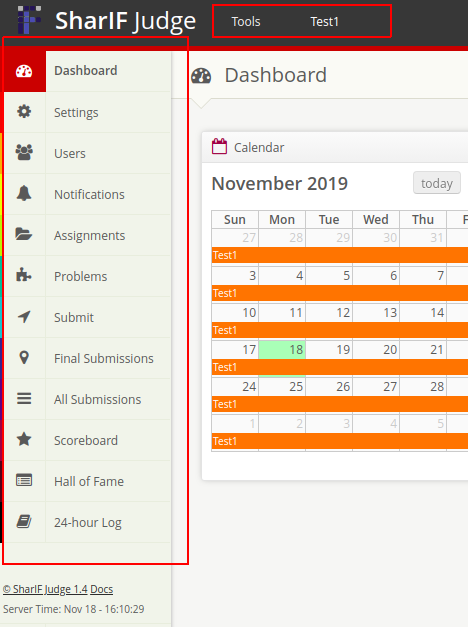
\includegraphics[scale=0.5]{kepatuhan_2_4_5}  
	\caption[Kriteria Sukses 2.4.5 - Menemukan Halaman Web Pada Navigasi]{Kriteria Sukses 2.4.5 - Menemukan Halaman Web Pada Navigasi} 
	\label{fig:kepatuhan_2_4_5} 
\end{figure}

\subsubsection{Kriteria Sukses 2.4.6 Headings and Labels}
\label{subsubsec:kepatuhan_kriteria_2.4.6}
(Tidak Sukses) \\

Kriteria ini tidak sukses dipatuhi karena :
\begin{itemize}
	\item Pada halaman \textit{Add User} ada \textit{field input} yang tidak memiliki label yang menjelaskan tujuannya. Pada potongan kode \ref{ls_kepatuhan_2_4_6_add_user} ada bidang masukan yang tidak memiliki label.
	\begin{lstlisting}[basicstyle=\ttfamily, frame=single,
	columns=fullflexible, keepspaces=true, breaklines=true, label=ls_kepatuhan_2_4_6_add_user, caption=Kriteria Sukses 2.4.6 - Halaman \textit{Add User}]
	...
	<p class="input_p">
		<textarea name="new_users" id="new_users" rows="20" cols="80" class="sharif_input">
		# Lines starting with a # sign are comments.
	...
	\end{lstlisting}
	
	\item Pada halaman \textit{Add Assignment} ada \textit{field input} yang tidak memiliki label yang menjelaskan tujuannya. Pada potongan kode \ref{ls_kepatuhan_2_4_6_add_assignment} ada bidang masukan yang tidak memiliki label.
	\begin{lstlisting}[basicstyle=\ttfamily, frame=single,
	columns=fullflexible, keepspaces=true, breaklines=true, label=ls_kepatuhan_2_4_6_add_assignment, caption=Kriteria Sukses 2.4.6 - Halaman \textit{Add Assignment}]
	...
	<td><input type="text" name="name[]" class="sharif_input short" value="{{ problem.name }}"/></td>
	...
	\end{lstlisting}
	
	\item Pada halaman \textit{Problems} bagian \textit{Edit Markdown} dan \textit{Edit Plain HTML} memiliki \textit{field input} yang tidak memiliki label yang menjelaskan tujuannya. Pada potongan kode \ref{ls_kepatuhan_2_4_6_edit_markdown} ada bidang masukan yang tidak memiliki label.
	\begin{lstlisting}[basicstyle=\ttfamily, frame=single,
	columns=fullflexible, keepspaces=true, breaklines=true, label=ls_kepatuhan_2_4_6_edit_markdown, caption=Kriteria Sukses 2.4.6 - Halaman \textit{Problems} bagian \textit{Edit Markdown}]
	...
	<p class="input_p">
		<textarea name="text">{{ problem.description }}</textarea>
	</p>
	...
	\end{lstlisting}
	
\end{itemize}

\subsubsection{Kriteria Sukses 2.4.7 Focus Visible}
\label{subsubsec:kepatuhan_kriteria_2.4.7}
(Tidak Sukses) \\

Kriteria ini tidak sukses dipatuhi karena fokus tidak tampak ketika fokus sedang berada pada menu \textit{sidebar}.

\subsubsection{Kriteria Sukses 2.4.8 Location}
\label{subsubsec:kepatuhan_kriteria_2.4.8}
(Sukses) \\

Kriteria ini sukses dipatuhi karena pada setiap halaman aplikasi \textit{SharIF Judge} terdapat judul yang menjelaskan lokasi pengguna.

\subsubsection{Kriteria Sukses 2.4.9 Link Purpose (Link Only)}
\label{subsubsec:kepatuhan_kriteria_2.4.9}
(Tidak Sukses) \\

Kriteria ini tidak sukses dipatuhi karena :
\begin{itemize}
	\item Pada halaman \textit{Assignment} ada gambar yang memiliki tautan tetapi tidak ada teks yang menjelaskan tujuan dari tautan tersebut. Pada potongan kode \ref{ls_kepatuhan_2_4_9_assignment} ditunjukkan bahwa gambar pdf memiliki tautan yang tidak memiliki teks yang menjelaskan tujuannya.
	\begin{lstlisting}[basicstyle=\ttfamily, frame=single,
	columns=fullflexible, keepspaces=true, breaklines=true, label=ls_kepatuhan_2_4_9_assignment, caption=Kriteria Sukses 2.4.9 - Gambar PDF]
	...
	<td>
	<a href="{{ site_url('assignments/pdf/'~item.id) }}"><img src="{{ base_url('assets/images/pdf.svg') }}" /></a>
	</td>
	...
	\end{lstlisting}
	
	\item Pada menu \textit{Top Bar} ada gambar yang memiliki tautan tetapi tidak ada teks yang menjelaskan tujuan dari tautan tersebut. Pada potongan kode \ref{ls_kepatuhan_2_4_9_top_bar} ditunjukkan bahwa gambar logo profil memiliki tautan yang tidak memiliki teks yang menjelaskan tujuannya.
	\begin{lstlisting}[basicstyle=\ttfamily, frame=single,
	columns=fullflexible, keepspaces=true, breaklines=true, label=ls_kepatuhan_2_4_9_top_bar, caption=Kriteria Sukses 2.4.9 - Gambar Logo Profile]
	...
	<a href="{{ site_url('profile') }}" id="profile_link"><i class="fa fa-user"></i></a>
	...
	\end{lstlisting}
	
\end{itemize}

\subsubsection{Kriteria Sukses 2.4.10 Section Headings}
\label{subsubsec:kepatuhan_kriteria_2.4.10}
(Tidak Sukses) \\

Kriteria ini tidak sukses dipatuhi karena pada aplikasi \textit{SharIF Judge} judul bagian tidak dipakai untuk mengatur konten. Pada potongan kode \ref{ls_kepatuhan_2_4_10_section_headings} bagian judul bagian tidak menggunakan tag \textit{heading}.
\begin{lstlisting}[basicstyle=\ttfamily, frame=single,
columns=fullflexible, keepspaces=true, breaklines=true, label=ls_kepatuhan_2_4_10_section_headings, caption=Kriteria Sukses 2.4.10 - Title Heading]
...
<div id="page_title">
	<i class="fa "></i>
	<span dir="auto"></span>
	
</div>
...
\end{lstlisting}

\subsubsection{Kriteria Sukses 2.5.1 Pointer Gestures}
\label{subsubsec:kepatuhan_kriteria_2.5.1}
(Sukses) \\

Kriteria ini sukses dipatuhi karena pada aplikasi \textit{SharIF Judge} tidak ada fungsionalitas yang harus dijalankan dengan menggunakan \textit{multipoint} atau gestur berbasis \textit{path}.

\subsubsection{Kriteria Sukses 2.5.2 Pointer Cancellation}
\label{subsubsec:kepatuhan_kriteria_2.5.2}
(Sukses) \\

Kriteria ini sukses dipatuhi karena pada aplikasi \textit{SharIF Judge} tidak ada fungsionalitas yang dapat dioperasikan dengan pointer tunggal dijalankan dengan menggunakan \textit{down-event}.

\subsubsection{Kriteria Sukses 2.5.3 Label in Name}
\label{subsubsec:kepatuhan_kriteria_2.5.3}
(Tidak Sukses) \\

Kriteria ini tidak sukses dipatuhi karena pada aplikasi \textit{SharIF Judge} masih banyak elemen yang tidak diberi label. Salah satu contohnya adalah halaman \textit{Problems} bagian \textit{Edit Markdown}. Tampilan halaman web dapat dilihat pada gambar \ref{fig:kepatuhan_2_5_3}.

\begin{figure}[H]
	\centering  
	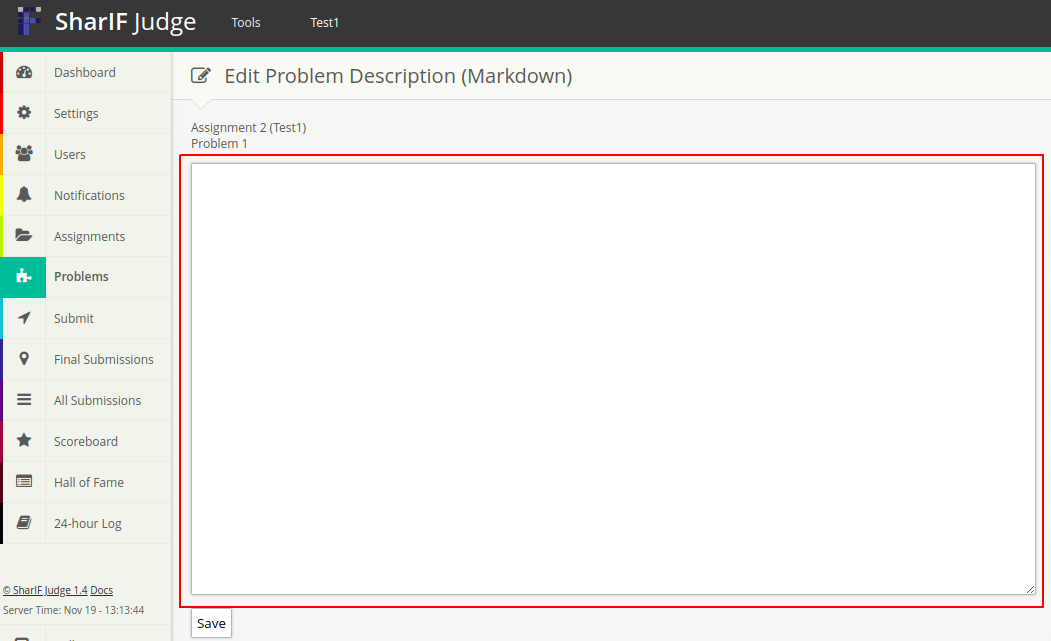
\includegraphics[scale=0.5]{kepatuhan_2_5_3}  
	\caption[Kriteria Sukses 2.5.3 - \textit{Edit Markdown}]{Kriteria Sukses 2.5.3 - \textit{Edit Markdown}} 
	\label{fig:kepatuhan_2_5_3} 
\end{figure}

\subsubsection{Kriteria Sukses 2.5.4 Motion Actuation}
\label{subsubsec:kepatuhan_kriteria_2.5.4}
(Sukses) \\

Kriteria ini sukses dipatuhi karena pada aplikasi \textit{SharIF Judge} tidak terdapat fungsionalitas yang dapat dioperasikan oleh gerakan perangkat atau gerakan pengguna.

\subsubsection{Kriteria Sukses 2.5.5 Target Size}
\label{subsubsec:kepatuhan_kriteria_2.5.5}
(Tidak Sukses) \\

Kriteria ini tidak sukses dipatuhi karena pada aplikasi \textit{SharIF Judge} masih banyak target yang dapat difokus berukuran kurang dari 44 piksel \textit{css}. Salah satu contohnya adalah bidang masukan \textit{Upload Size Limit} yang berukuran 30 piksel css. Tampilan halaman web dapat dilihat pada gambar \ref{fig:kepatuhan_2_5_5}.

\begin{figure}[H]
	\centering  
	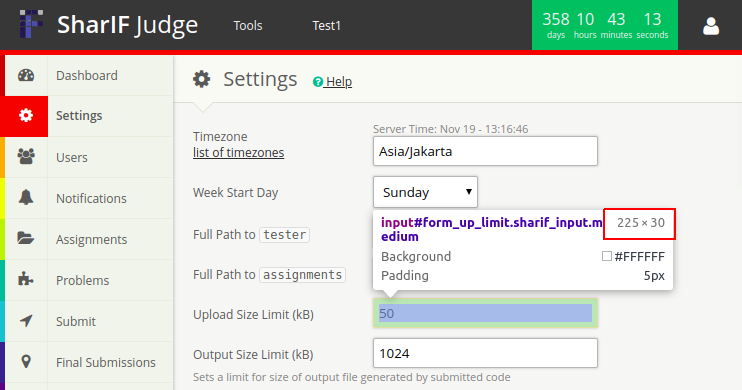
\includegraphics[scale=0.5]{kepatuhan_2_5_5}  
	\caption[Kriteria Sukses 2.5.5 - Bidang Masukan Berukuran 30 css Piksel]{Kriteria Sukses 2.5.5 - Bidang Masukan Berukuran 30 css Piksel} 
	\label{fig:kepatuhan_2_5_5} 
\end{figure}

\subsubsection{Kriteria Sukses 2.5.6 Concurrent Input Mechanisms}
\label{subsubsec:kepatuhan_kriteria_2.5.6}
(Sukses) \\

Kriteria ini sukses dipatuhi karena pada aplikasi \textit{SharIF Judge} tidak membatasi modalitas masukan yang tersedia pada platform.

\subsection{\textit{Understandable}}
\label{subsec:kepatuhan_understandable}

\subsubsection{Kriteria Sukses 3.1.1 Language of Page}
\label{subsubsec:kepatuhan_kriteria_3.1.1}
(Tidak Sukses) \\

Kriteria ini tidak sukses dipatuhi karena elemen \textit{html} tidak memiliki atribut \textit{lang}. Pada potongan kode \ref{ls_kepatuhan_3_1_1} ditunjukkan bahwa elemen \textit{html} tidak memiliki atribut \textit{lang}.
\begin{lstlisting}[basicstyle=\ttfamily, frame=single,
columns=fullflexible, keepspaces=true, breaklines=true, label=ls_kepatuhan_3_1_1, caption=Kriteria Sukses 3.1.1 - Elemen \textit{HTML}]
...
<html>
<head>
...
\end{lstlisting}

\subsubsection{Kriteria Sukses 3.1.2 Language of Parts}
\label{subsubsec:kepatuhan_kriteria_3.1.2}
(Tidak Sukses) \\

Kriteria ini tidak sukses dipatuhi karena elemen \textit{html} tidak memiliki atribut \textit{lang}. Semua halaman pada aplikasi \textit{SharIF Judge} memakai bahasa Inggris, jika elemen \textit{html} memiliki atribut \textit{lang} maka kriteria ini akan terpenuhi.

\subsubsection{Kriteria Sukses 3.1.3 Unusual Words}
\label{subsubsec:kepatuhan_kriteria_3.1.3}
(Sukses) \\

Kriteria ini sukses dipatuhi karena pada aplikasi \textit{SharIF Judge} tidak ada kata atau frasa tertentu yang digunakan dengan cara tidak biasa atau terbatas. 

\subsubsection{Kriteria Sukses 3.1.4 Abbreviations}
\label{subsubsec:kepatuhan_kriteria_3.1.4}
(Sukses) \\

Kriteria ini sukses dipatuhi karena singkatan yang ada pada \textit{SharIF Judge} lazim digunakan oleh kalangan informatika, singkatan yang dimaksud adalah IP, PDF.

\subsubsection{Kriteria Sukses 3.1.5 Reading Level}
\label{subsubsec:kepatuhan_kriteria_3.1.5}
(Sukses) \\

Kriteria ini sukses dipatuhi karena pada aplikasi \textit{SharIF Judge} tidak ada teks yang membutuhkan kemampuan membaca lebih maju daripada tingkat pendidikan menengah bawah.

\subsubsection{Kriteria Sukses 3.1.6 Pronunciation}
\label{subsubsec:kepatuhan_kriteria_3.1.6}
(Sukses) \\

Kriteria ini sukses dipatuhi karena pada halaman aplikasi \textit{SharIF Judge} setiap kata dapat dimengerti artinya tanpa pengguna perlu mengetahui cara mengucapkan kata tersebut.

\subsubsection{Kriteria Sukses 3.2.1 On Focus}
\label{subsubsec:kepatuhan_kriteria_3.2.1}
(Sukses) \\

Kriteria ini sukses dipatuhi karena pada halaman aplikasi \textit{SharIF Judge} setiap komponen antarmuka yang menerima fokus tidak menyebabkan perubahan konteks.

\subsubsection{Kriteria Sukses 3.2.2 On Input}
\label{subsubsec:kepatuhan_kriteria_3.2.2}
(Sukses) \\

Kriteria ini sukses dipatuhi karena pada setiap pengguna mengubah setelan komponen antarmuka tidak menyebabkan perubahan konteks.

\subsubsection{Kriteria Sukses 3.2.3 Consistent Navigation}
\label{subsubsec:kepatuhan_kriteria_3.2.3}
(Sukses) \\

Kriteria ini sukses dipatuhi karena bagian navigasi menu yang muncul berulang pada tiap halaman aplikasi \textit{SharIF Judge}, muncul dalam urutan relatif yang sama setiap kali terlihat.

\subsubsection{Kriteria Sukses 3.2.4 Consistent Identification}
\label{subsubsec:kepatuhan_kriteria_3.2.4}
(Tidak Sukses) \\

Kriteria ini tidak sukses dipatuhi karena ada komponen yang memiliki fungsi yang sama tetapi tidak diidentifikasi secara konsisten. Komponen tersebut antara lain :

\begin{itemize}
	\item Pada halaman \textit{Assignments} istilah untuk menambah \textit{Assignment} diberi nama \textit{Add}. Tampilan halaman web dapat dilihat pada gambar \ref{fig:kepatuhan_3_2_4_assignments}.
	\begin{figure}[H]
		\centering  
		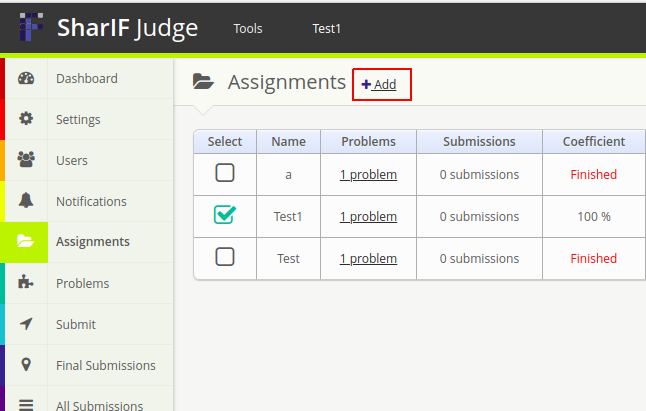
\includegraphics[scale=0.5]{kepatuhan_3_2_4_assignments}  
		\caption[Kriteria Sukses 3.2.4 - \textit{Assignments}]{Kriteria Sukses 3.2.4 - \textit{Assignments}} 
		\label{fig:kepatuhan_3_2_4_assignments} 
	\end{figure}

	\item Pada halaman \textit{Users} istilah untuk menambah \textit{user} diberi nama \textit{Add User}. Tampilan halaman web dapat dilihat pada gambar \ref{fig:kepatuhan_3_2_4_users}.
	\begin{figure}[H]
		\centering  
		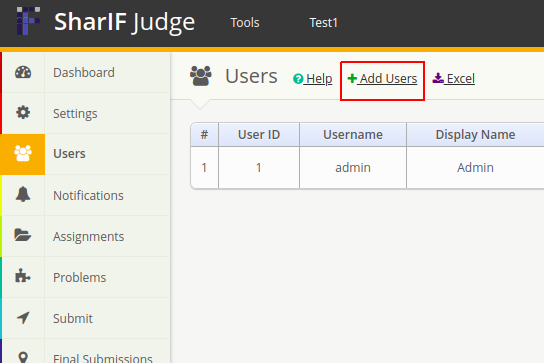
\includegraphics[scale=0.5]{kepatuhan_3_2_4_users}  
		\caption[Kriteria Sukses 3.2.4 - \textit{Users}]{Kriteria Sukses 3.2.4 - \textit{Users}} 
		\label{fig:kepatuhan_3_2_4_users} 
	\end{figure}

	\item Pada halaman. \textit{Notifications} istilah untuk menambah \textit{Notification} diberi nama \textit{New}. Tampilan halaman web dapat dilihat pada gambar \ref{fig:kepatuhan_3_2_4_notifications}.
	\begin{figure}[H]
		\centering  
		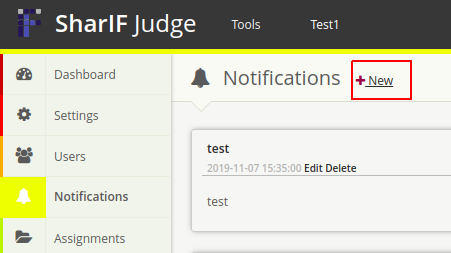
\includegraphics[scale=0.5]{kepatuhan_3_2_4_notifications}  
		\caption[Kriteria Sukses 3.2.4 - \textit{Notifications}]{Kriteria Sukses 3.2.4 - \textit{Notifications}} 
		\label{fig:kepatuhan_3_2_4_notifications} 
	\end{figure}

\end{itemize}

\subsubsection{Kriteria Sukses 3.2.5 Change on Request}
\label{subsubsec:kepatuhan_kriteria_3.2.5}
(Sukses) \\

Kriteria ini sukses dipatuhi karena perubahan konteks hanya terjadi bila dilakukan oleh pengguna.

\subsubsection{Kriteria Sukses 3.3.1 Error Identification}
\label{subsubsec:kepatuhan_kriteria_3.3.1}
(Sukses)\\

Kriteria ini sukses dipatuhi karena kesalahan masukan terdeteksi secara otomatis, \textit{item} yang salah diidentifikasi dan kesalahan tersebut dijelaskan kepada pengguna dalam teks.

\subsubsection{Kriteria Sukses 3.3.2 Labels or Instructions}
\label{subsubsec:kepatuhan_kriteria_3.3.2}
(Tidak Sukses) \\

Kriteria ini tidak sukses karena pada halaman problem bagian edit html, edit markdown, dan edit plain html tidak ada label atau instruksi untuk pengisiannya. Salah satu contoh tampilan halaman web dapat dilihat pada gambar \ref{fig:kepatuhan_3_3_2_edit_markdown}.
\begin{figure}[H]
	\centering  
	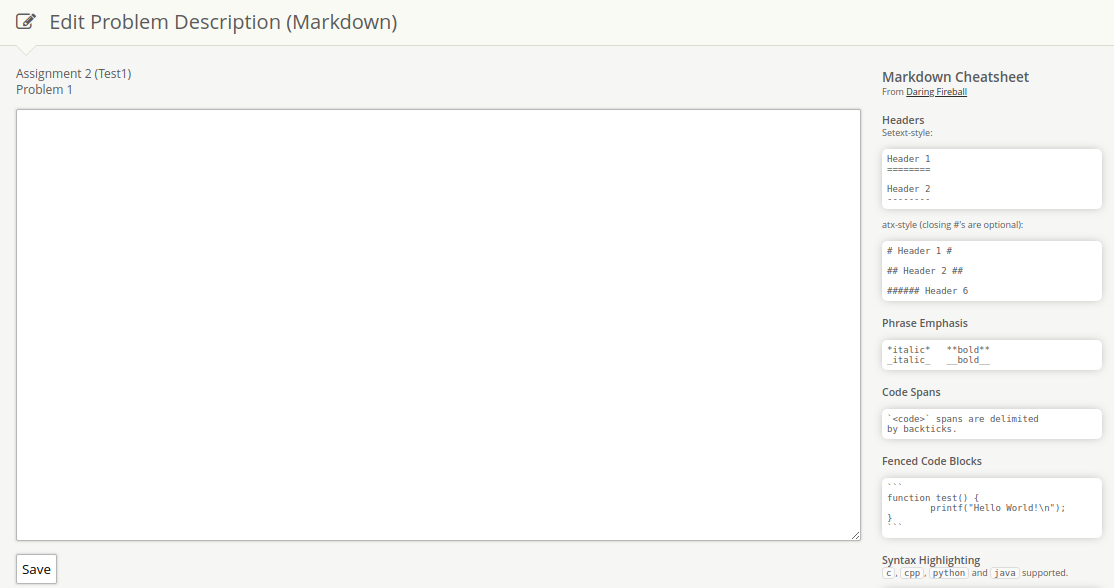
\includegraphics[scale=0.25]{kepatuhan_3_3_2_edit_markdown}  
	\caption[Kriteria Sukses 3.3.2 - \textit{Edit Markdown} Tidak Diberi Label Atau Instruksi]{Kriteria Sukses 3.3.2 - \textit{Edit Markdown} Tidak Diberi Label Atau Instruksi} 
	\label{fig:kepatuhan_3_3_2_edit_markdown} 
\end{figure}

\subsubsection{Kriteria Sukses 3.3.3 Error Suggestion}
\label{subsubsec:kepatuhan_kriteria_3.3.3}
(Sukses) \\

Kriteria ini sukses dipatuhi karena ketika kesalahan masukan terdeteksi secara otomatis dan saran untuk mengoreksi diketahui, maka saran tersebut diberikan kepada pengguna.

\subsubsection{Kriteria Sukses 3.3.4 Error Prevention (Legal, Financial, Data)}
\label{subsubsec:kepatuhan_kriteria_3.3.4}
(Sukses) \\

Kriteria ini sukses dipatuhi karena pada halaman yang mengirim tanggapan pengguna, data yang dimasukkan oleh pengguna diperiksa terkait kesalahan masukan dan pengguna dipersilakan untuk mengoreksinya.

\subsubsection{Kriteria Sukses 3.3.5 Help}
\label{subsubsec:kepatuhan_kriteria_3.3.5}
(Tidak Sukses) \\

Kriteria ini tidak sukses dipatuhi karena
pada aplikasi \textit{SharIF Judge} masih ada konten yang tidak diberi label. Pengguna harus dapat mengetahui tujuan dari konten melalui labelnya.

\subsubsection{Kriteria Sukses 3.3.6 Error Prevention (All)}
\label{subsubsec:kepatuhan_kriteria_3.3.6}
(Sukses) \\

Kriteria ini sukses dipatuhi karena pada halaman yang mengharuskan pengguna untuk mengirimkan informasi, data yang dimasukkan oleh pengguna diperiksa terkait kesalahan masukan dan pengguna dipersilakan untuk mengoreksinya.

\subsection{\textit{Robust}}
\label{subsec:kepatuhan_robust}

\subsubsection{Kriteria Sukses 4.1.1 Parsing}
\label{subsubsec:kepatuhan_kriteria_4.1.1}

\subsubsection{Kriteria Sukses 4.1.2 Name, Role, Value}
\label{subsubsec:kepatuhan_kriteria_4.1.2}
(Tidak Sukses) \\

Kriteria ini tidak sukses dipatuhi karena : 
\begin{itemize}
	\item Teknologi bantuan tidak dapat mengambil informasi pada \textit{sidebar} karena tidak ada teks yang menjelaskan link tersebut.
\end{itemize}

\subsubsection{Kriteria Sukses 4.1.3 Status Messages}
\label{subsubsec:kepatuhan_kriteria_4.1.3}
(Tidak Sukses) \\

Kriteria ini tidak sukses dipatuhi karena pada aplikasi \textit{SharIF Judge} tidak ada notifikasi saat melakukan aksi.